\documentclass[12pt]{article}
\usepackage{sbc-template}
\usepackage{graphicx,url}
\usepackage[brazil]{babel}   
\usepackage[utf8]{inputenc}  
\usepackage{placeins}
\usepackage{graphicx}


\sloppy

\title{Interação Humano-computador:\\Atividades baseadas em um projeto de site de venda de ingressos}

\author{
    \begin{minipage}{\textwidth}
        Carlos Alberto\inst{1},
        Daniela Menezes\inst{2},
        Danilo Caldeira\inst{3},
        Gabriel Augusto R. dos Reis\inst{4},
        Giovani Araújo\inst{5},
        Giovanna Badaró\inst{6},
        Guilherme Ferreira Faioli Lima\inst{7},
        Indianara Santos Rodrigues\inst{8},
        Luiz Carlos Silva Júnior\inst{9}
    \end{minipage}
}

\address{
Departamento de Computação e Sistemas\\
Universidade Federal de Ouro Preto (UFOP) -- João Monlevade, MG \\
\\  16.2.8394 \inst{1},
    16.2.8540 \inst{2},
    16.2.8512 \inst{3},
    16.2.8105\inst{4},
    16.2.8149 \inst{5},
    14.2.8384 \inst{6},
    16.1.8243 \inst{7},\\
    17.2.8246 \inst{8},
    15.1.5881\inst{9}
}

\begin{document} 

\maketitle

\begin{abstract}
Consists of a set of activities related to each other, in the area of software engineering, relating parts of a software development process, the main mechanism to obtain quality software, fulfilling the stages of development of a web site project for software events.
\end{abstract}
     
\begin{resumo}
Consiste num conjunto de atividades relacionadas entre sí, na área de engenharia de software, relatando partes de um processo de desenvolvimento de software, principal mecanismo para se obter software de qualidade, cumprindo as etapas do desenvolvimento de um projeto de site de vendas de ingressos para eventos.
\end{resumo}

\tableofcontents
\newpage

\section{Casos de Uso}
    \begin{enumerate}
        \item Compra de ingressos \\
        Quando já definido o evento desejado, o usuário realiza a solicitação de compra do ingresso. Caso não seja um usuário cadastrado, deverá se cadastrar. Quando já cadastrado, é redirecionado para a confirmação do pagamento (cartão de crédito/débito/boleto/voucher) e validado pelo sistema e enviado para o e-mail cadastrado um código de confirmação.
        \item Alteração de ingresso \\
        Após a realização da compra do ingresso, o cliente pode solicitar a alteração do ingresso, até 24 horas antes do evento. Quando dentro das conformidades, é gerado um novo ingresso com as alterações requisitadas.
        \item Cancelamento de ingressos \\
        O cliente tem a opção solicitar o cancelamento de sua compra, até 24 horas antes do evento. Sendo assim é analisado e contabilizado no sistema, podendo ser feito o estorno (no caso de compras no cartão), ou devolução do dinheiro no caso seja boleto ou compra presencial.
        \item Gestão de Vendas \\
        O sistema gera relatórios de pós-venda. Emite informações em tempo real de vendas (demanda do público alvo, repercussão em redes sociais). Emite relatórios inteligentes. 
        \item Retirada de ingressos \\
        Após a confirmação da compra do ingresso, o cliente pode fazer a retirada diretamente na bilheteria apresentando um código e seus documentos ou fazer impressão do ingresso que será enviado em seu e-mail.
        \item Pesquisar \\
        O usuário tem a opção de buscar o evento através de filtros: região, tipo, data e horário, local do evento.
        \item Administrar conta \\
        O usuário pode criar conta, editar conta, colocar foto, verificar ingressos comprados, informações dos ingressos, alterar dados de pagamento.
        \item Publicar eventos \\
        O organizador deverá solicitar o sistema autorização para criar um evento com o nome, a data, o tipo do ingresso (pago, gratuito), local, descrição do evento (programação e detalhes) e informações sobre o organizador. 
        \item Atendimento \\
        O usuário tem a opção de entrar contato com o sistema de compras através de redes sociais, tais como: Instagram e Facebook. Através de e-mail, telefone e chat online. 
    \end{enumerate}

\section{Modelo de domínio}
    
    \begin{figure}[h]
        \centering
        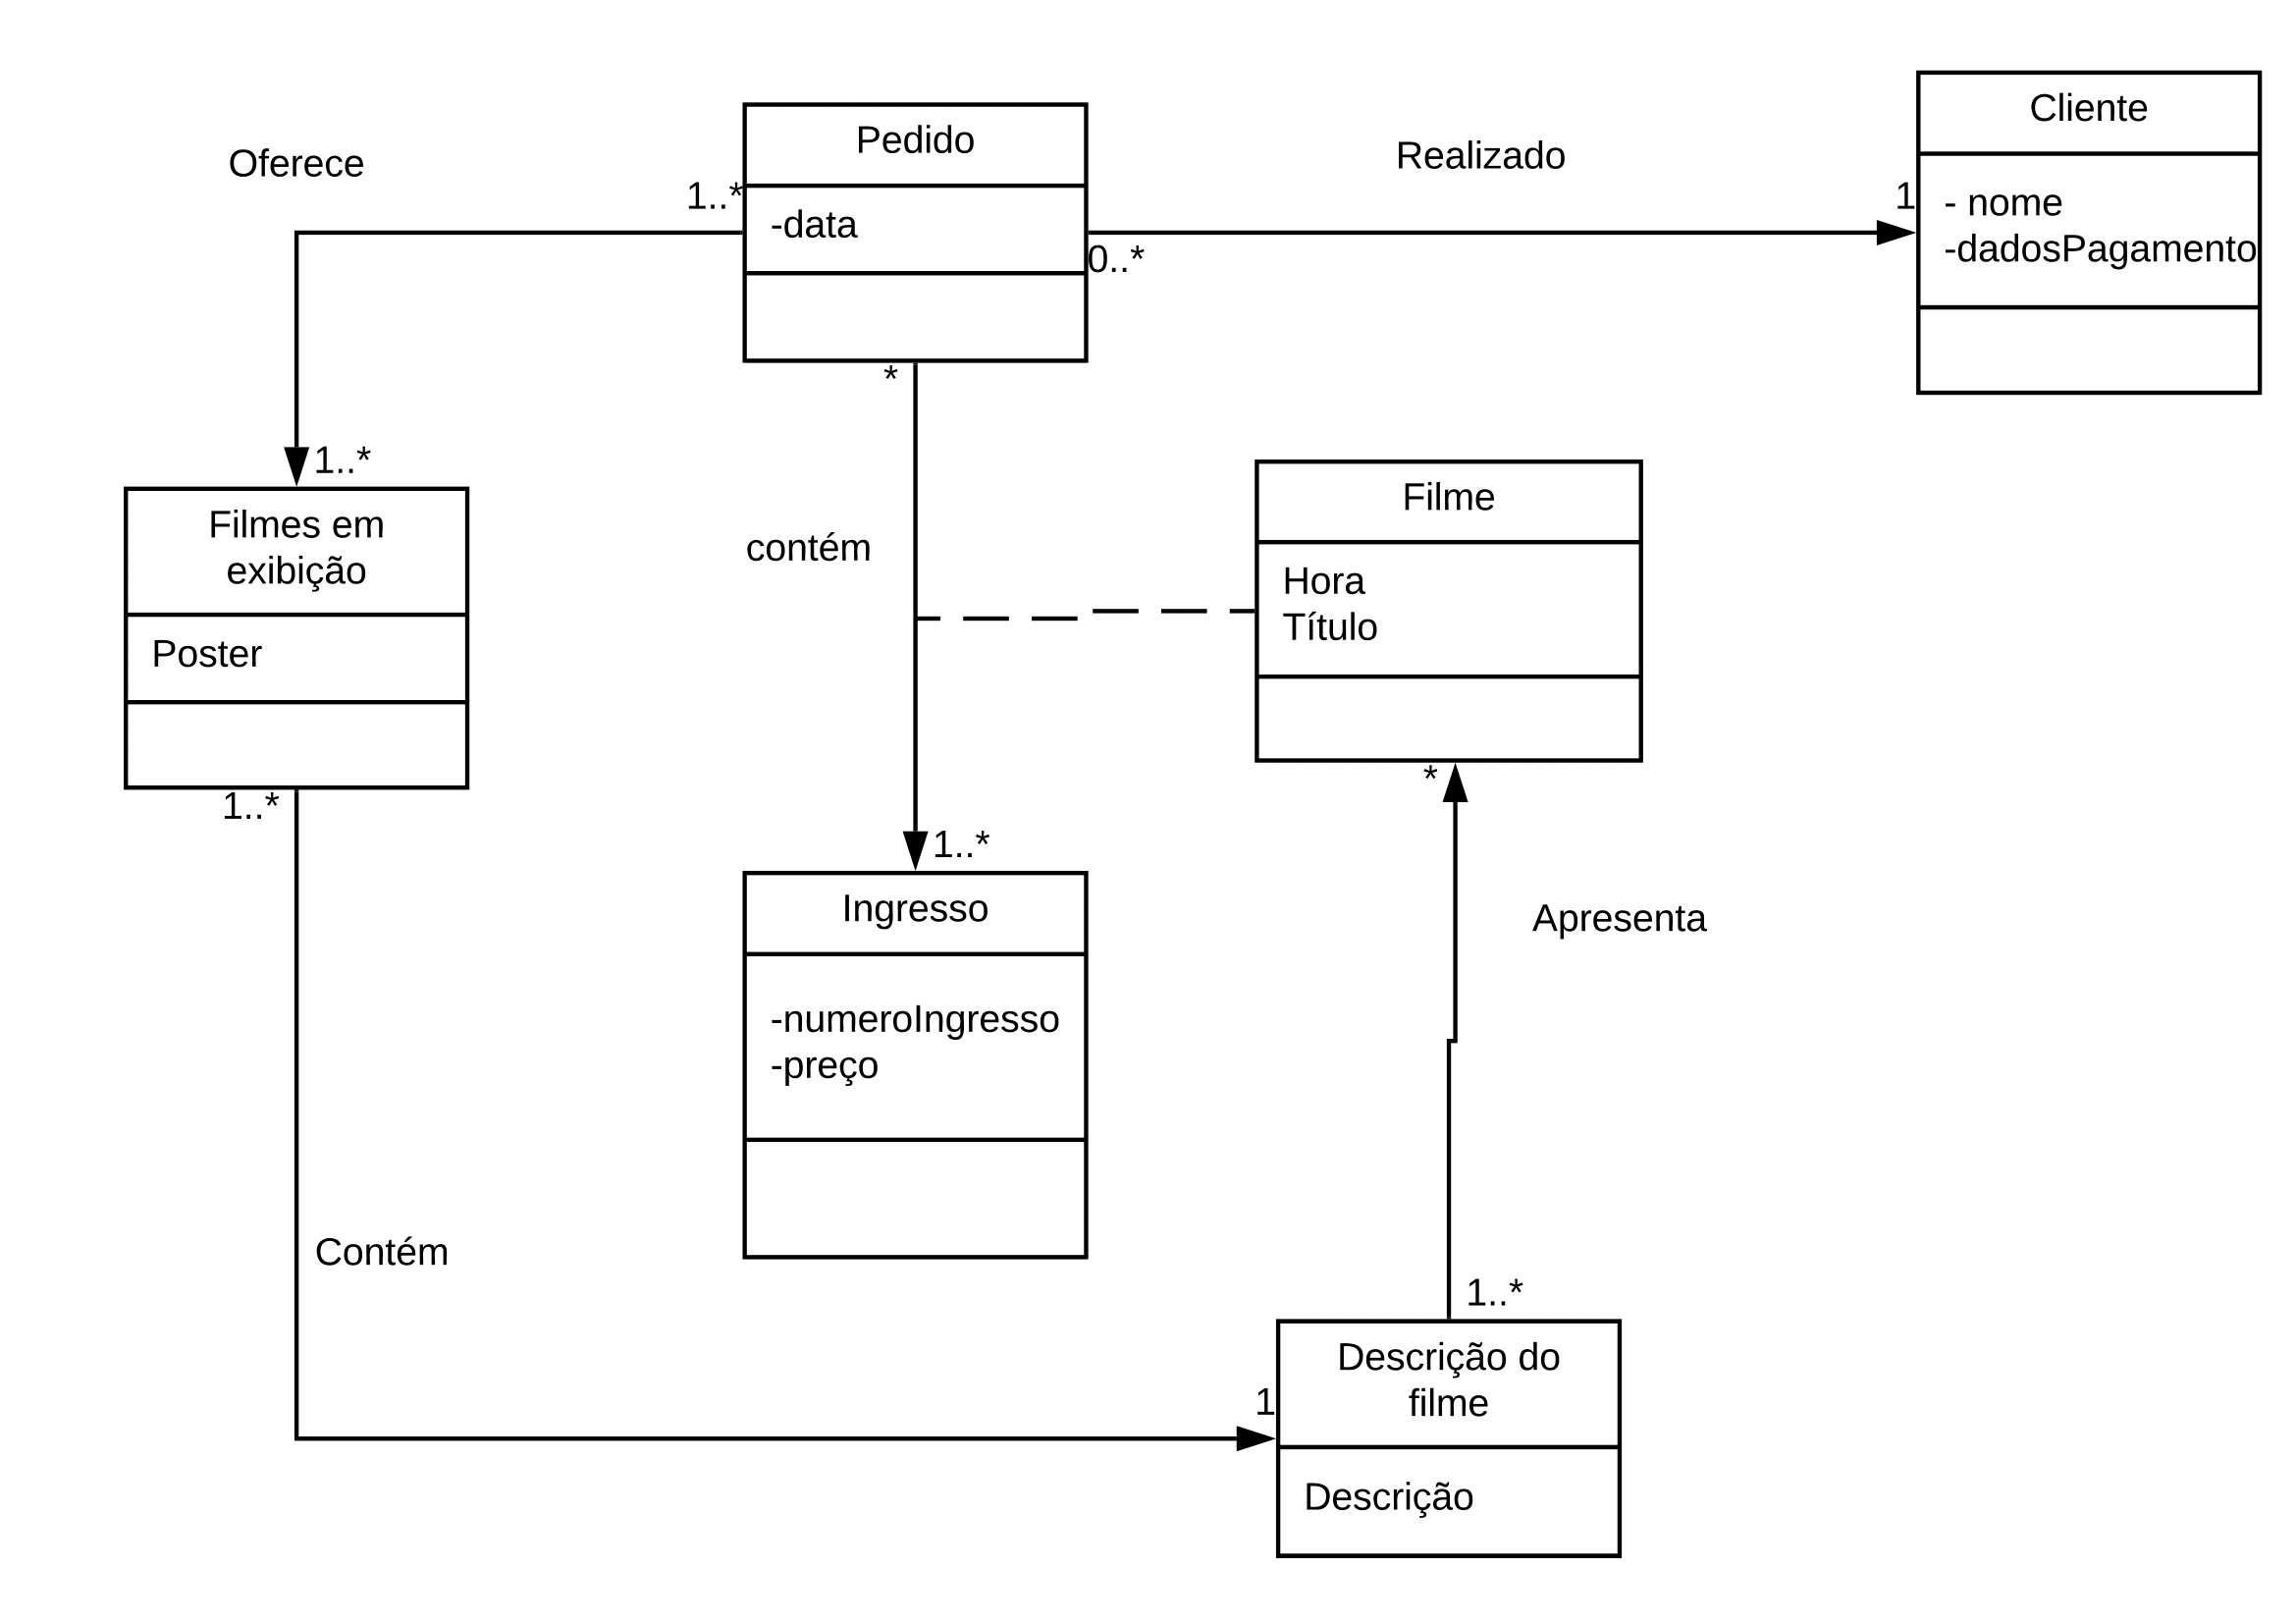
\includegraphics[scale=0.18]{./Imagens/ModeloDeDominio.png}
        \caption{Modelo de domínio}
        \label{fig:ModeloDeDominio}
    \end{figure}
    \FloatBarrier

\section{Diagramas de Sequencia de Sistema}

    \begin{figure}[h]
        \centering
        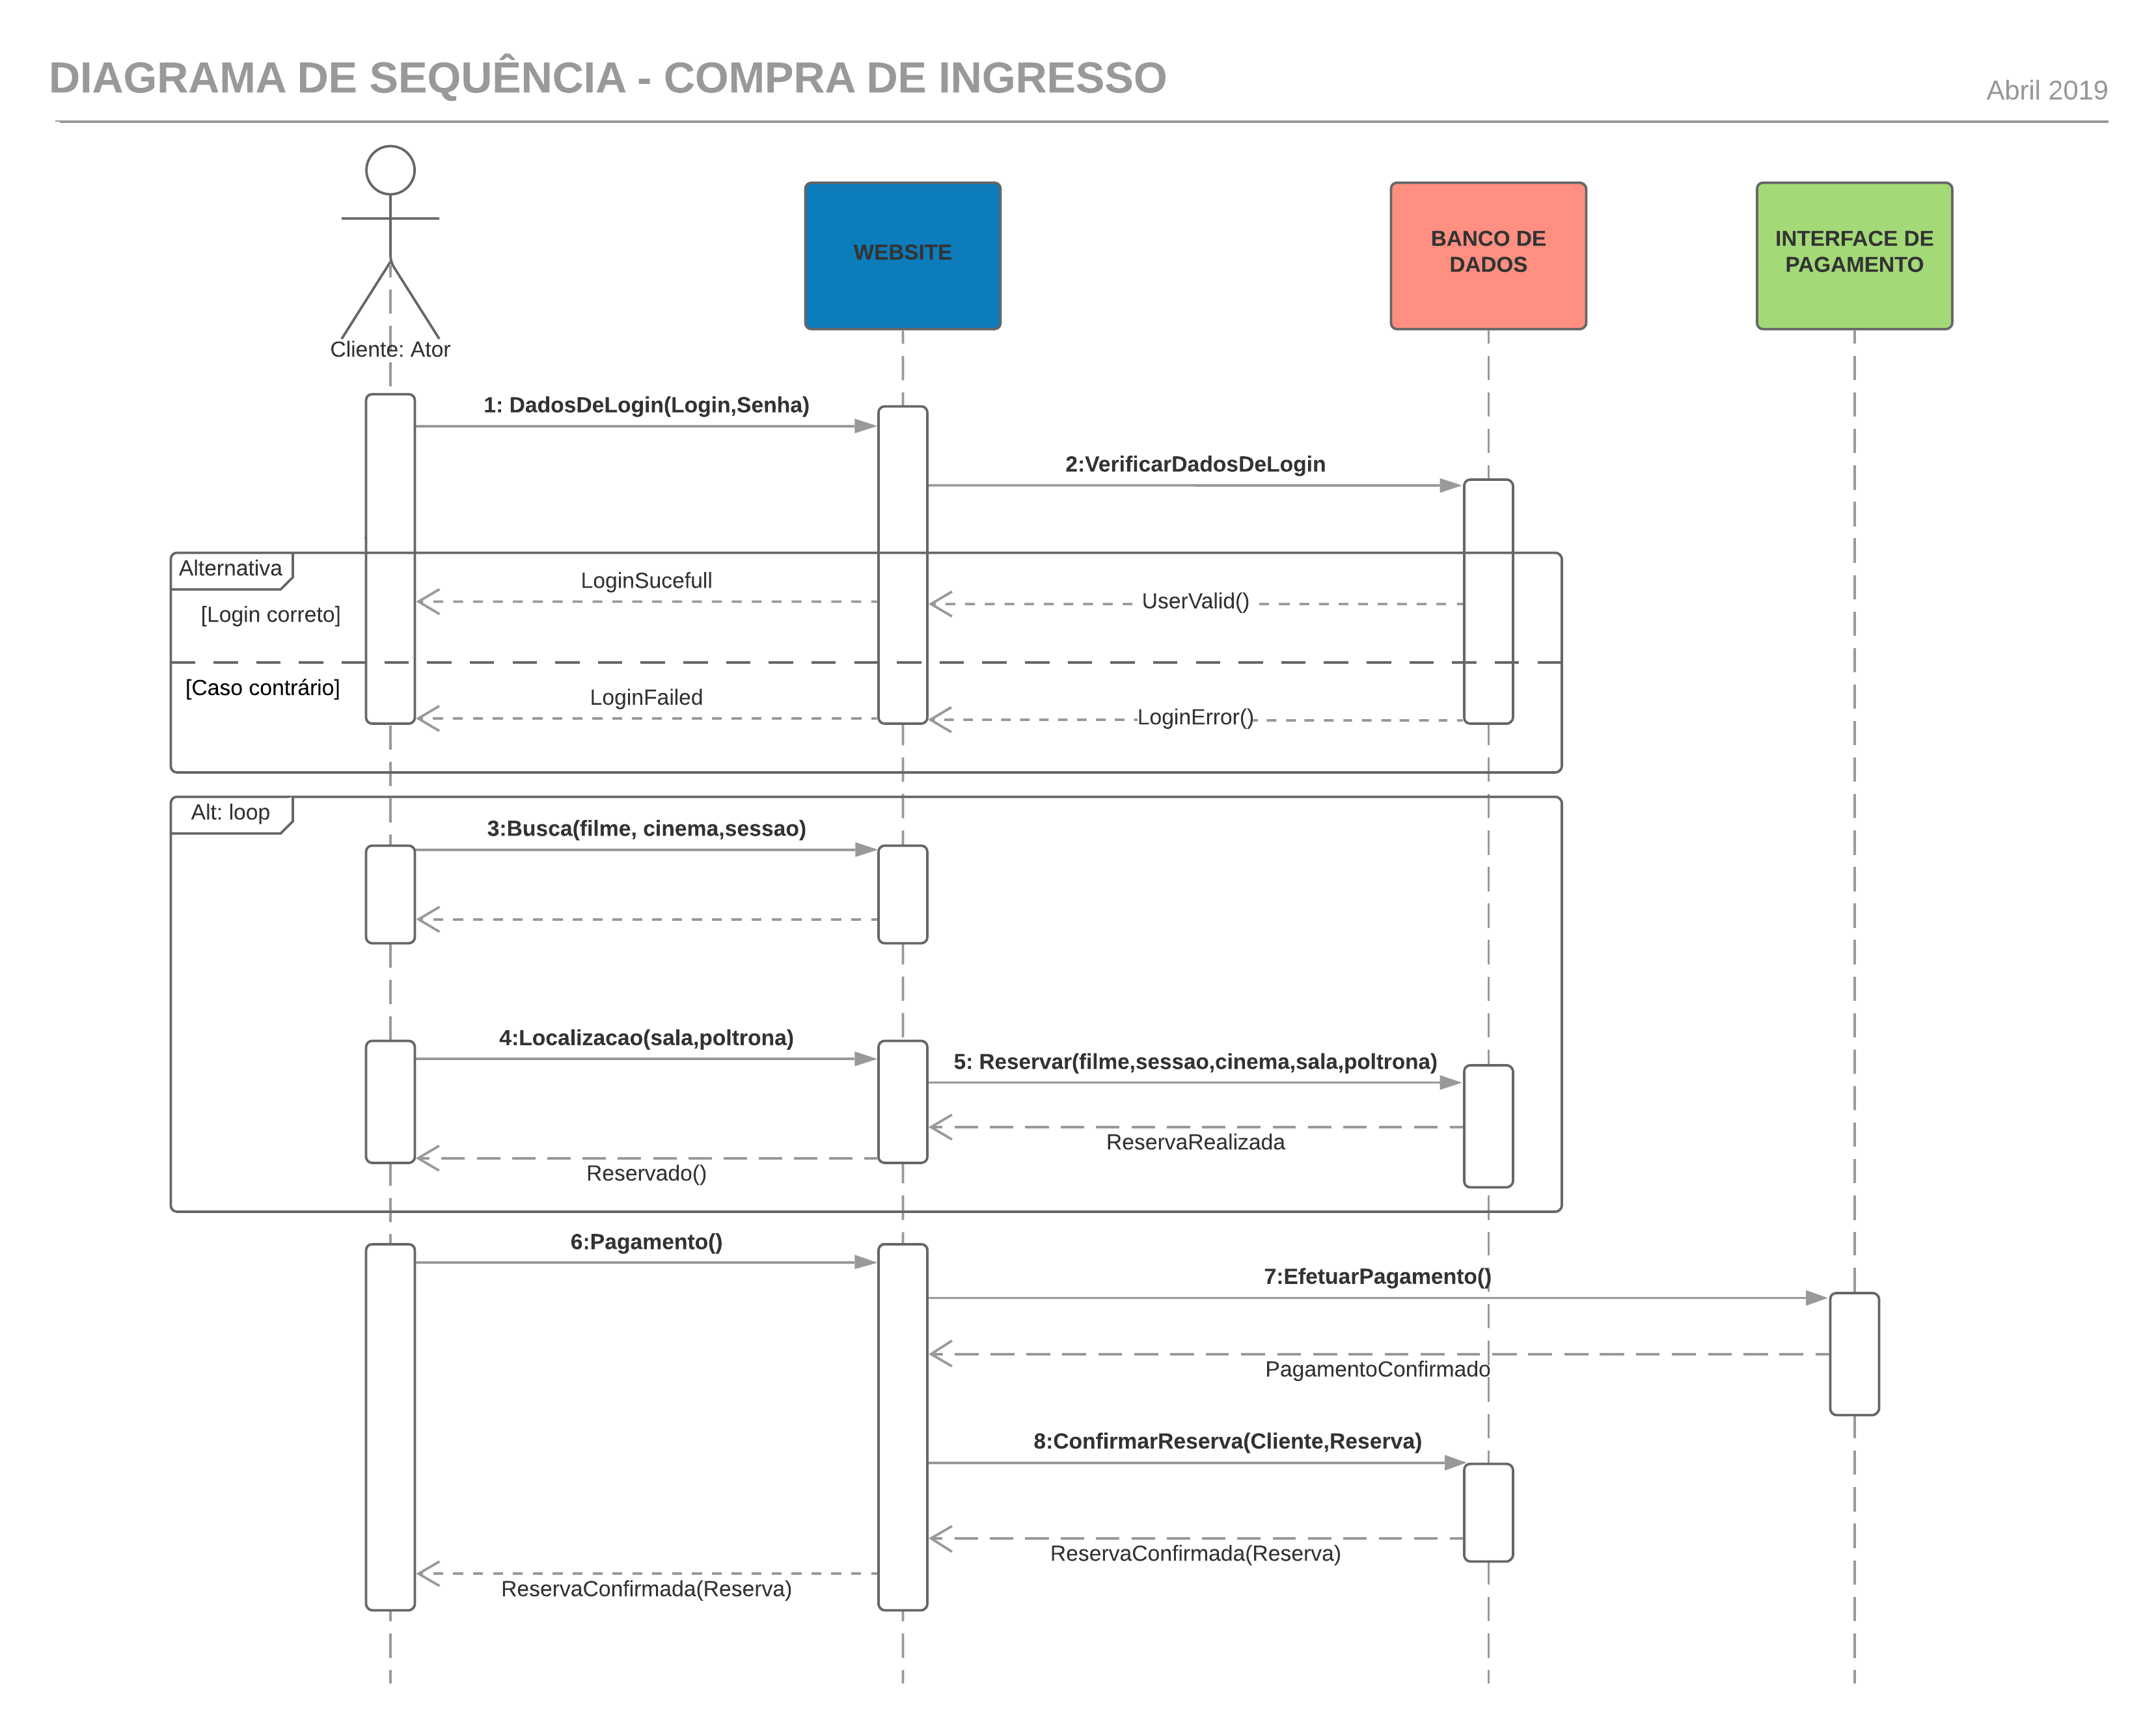
\includegraphics[scale=0.5]{./Imagens/DiagramasDeSequencia/DiagramaDeSequencia1.png}
        \caption{Diagrama de sequencia - Compra de ingressos}
        \label{fig:DiagramaSequencia01}
    \end{figure}

    \begin{figure}[h]
        \centering
        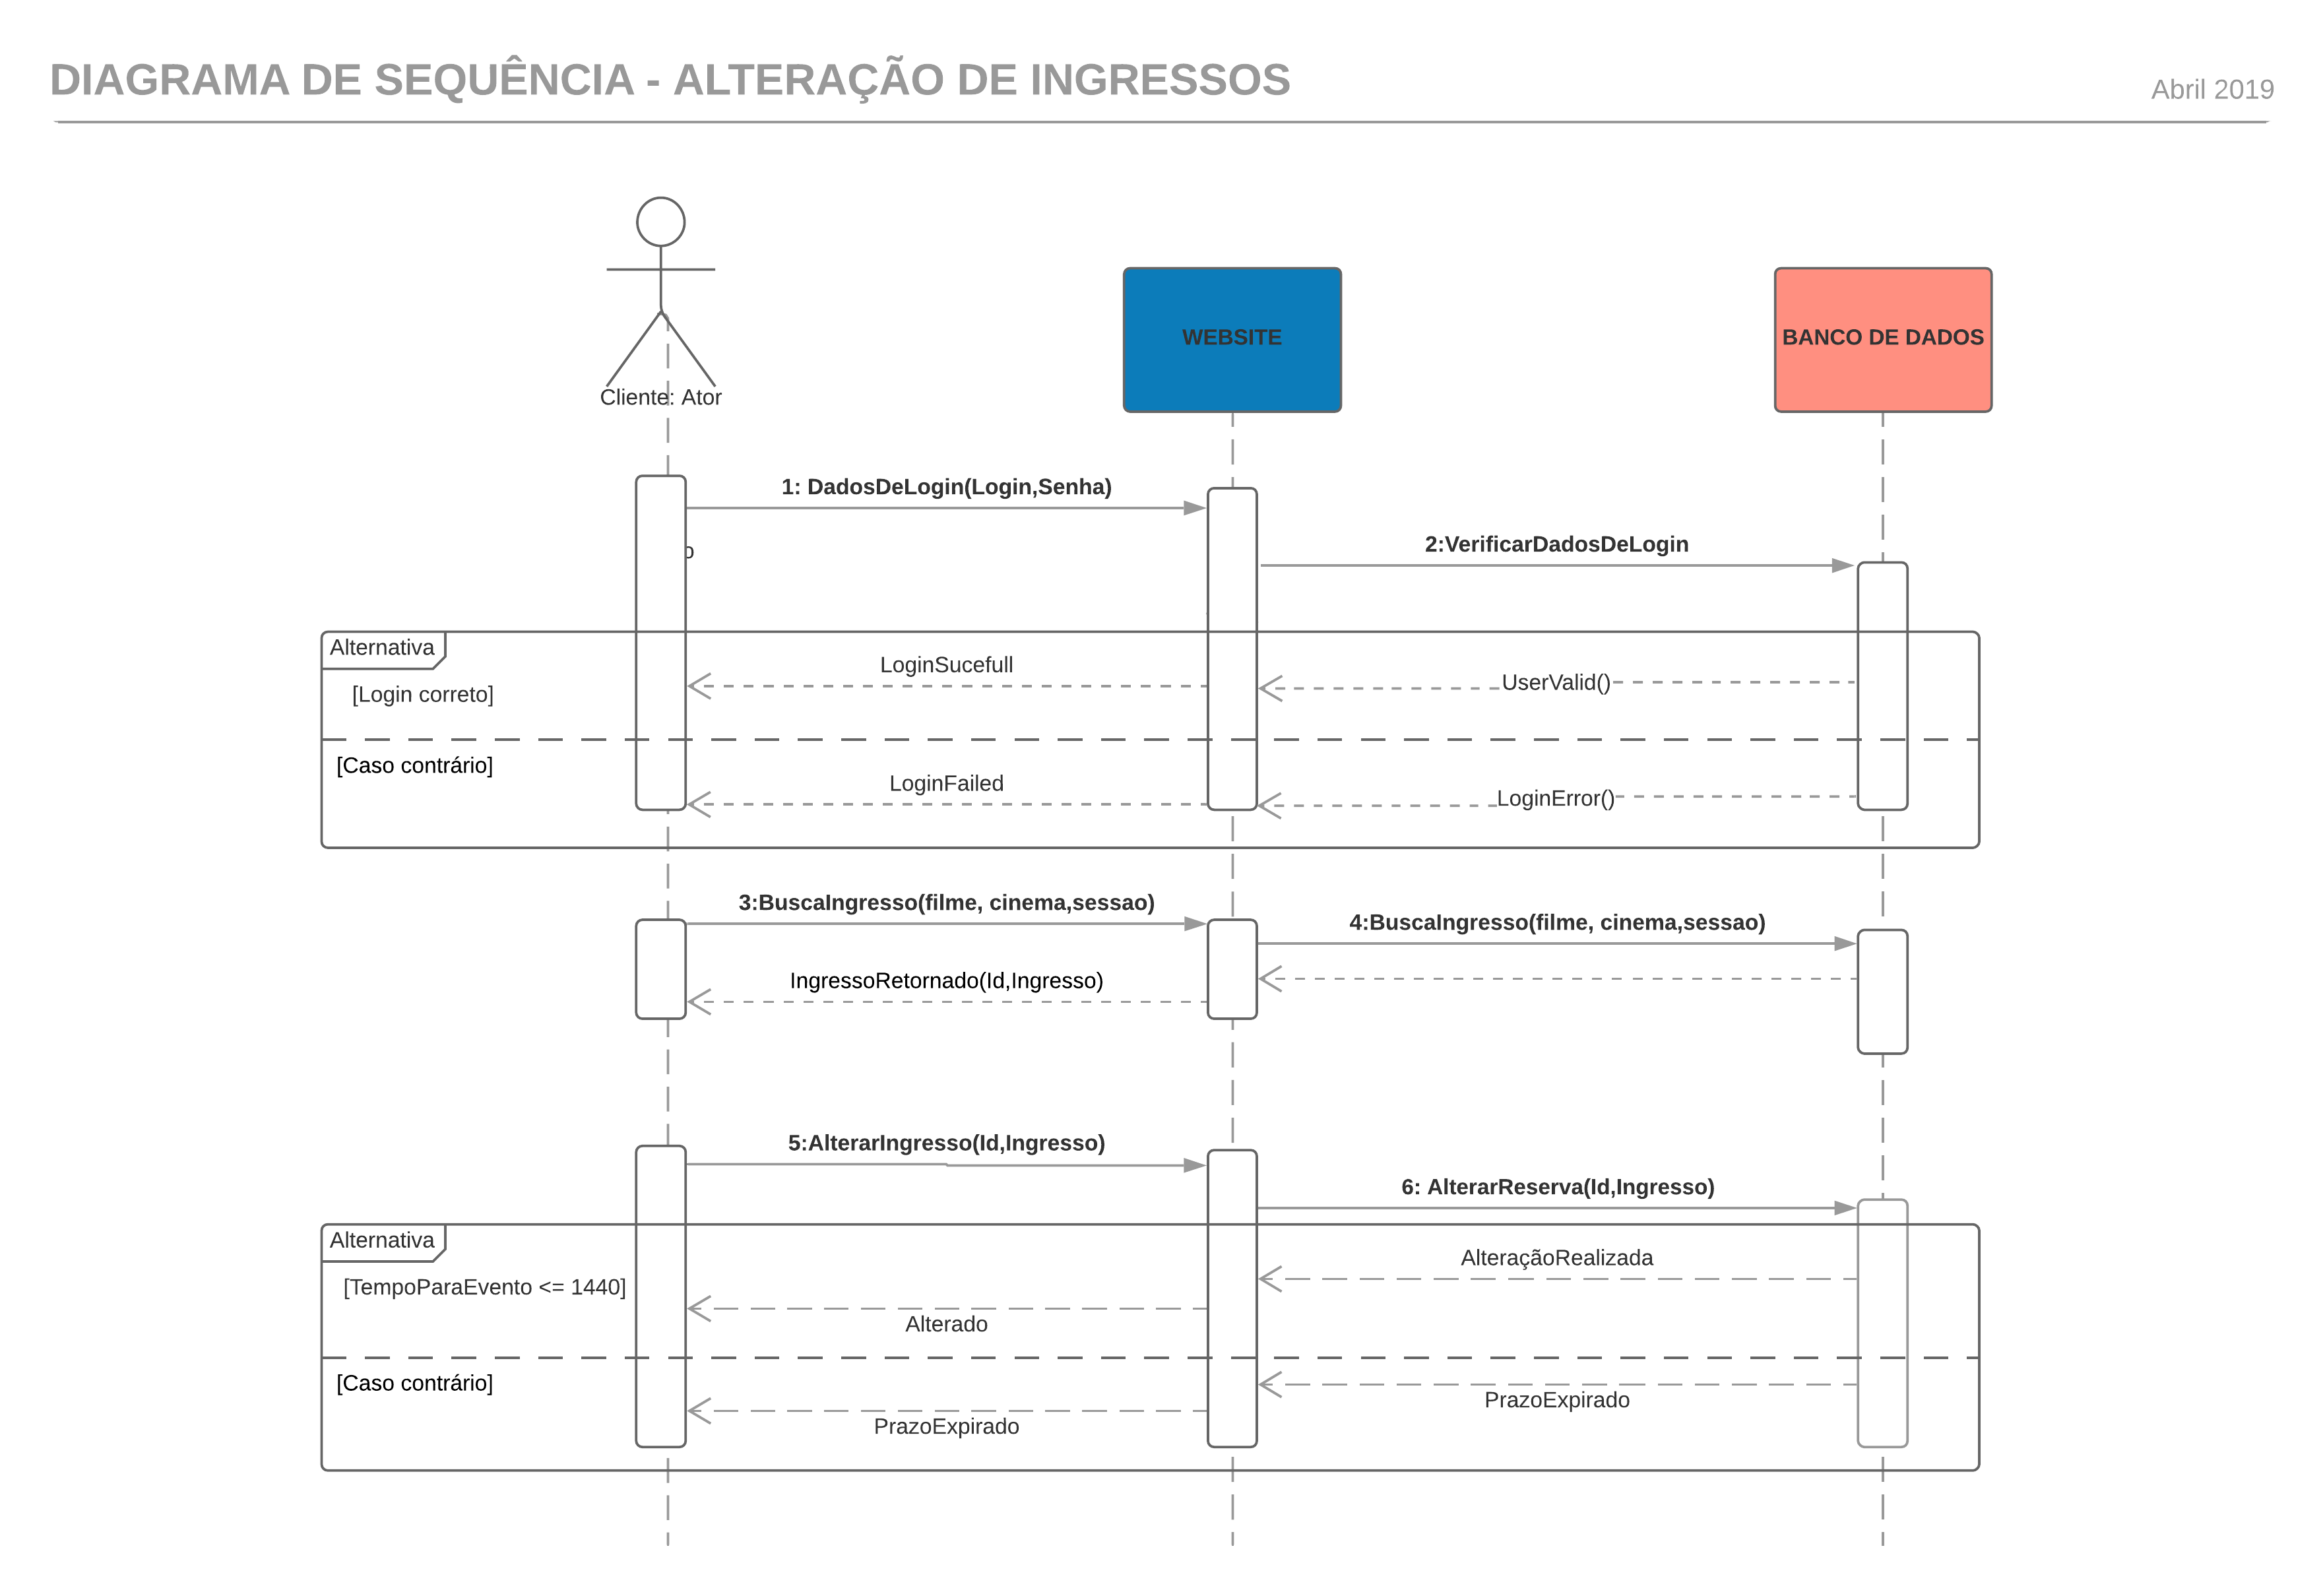
\includegraphics[scale=0.5]{./Imagens/DiagramasDeSequencia/DiagramaDeSequencia2.png}
        \caption{Diagrama de sequencia - Alteração de ingressos}
        \label{fig:DiagramaSequencia02}
    \end{figure}
   
    \begin{figure}[h]
        \centering
        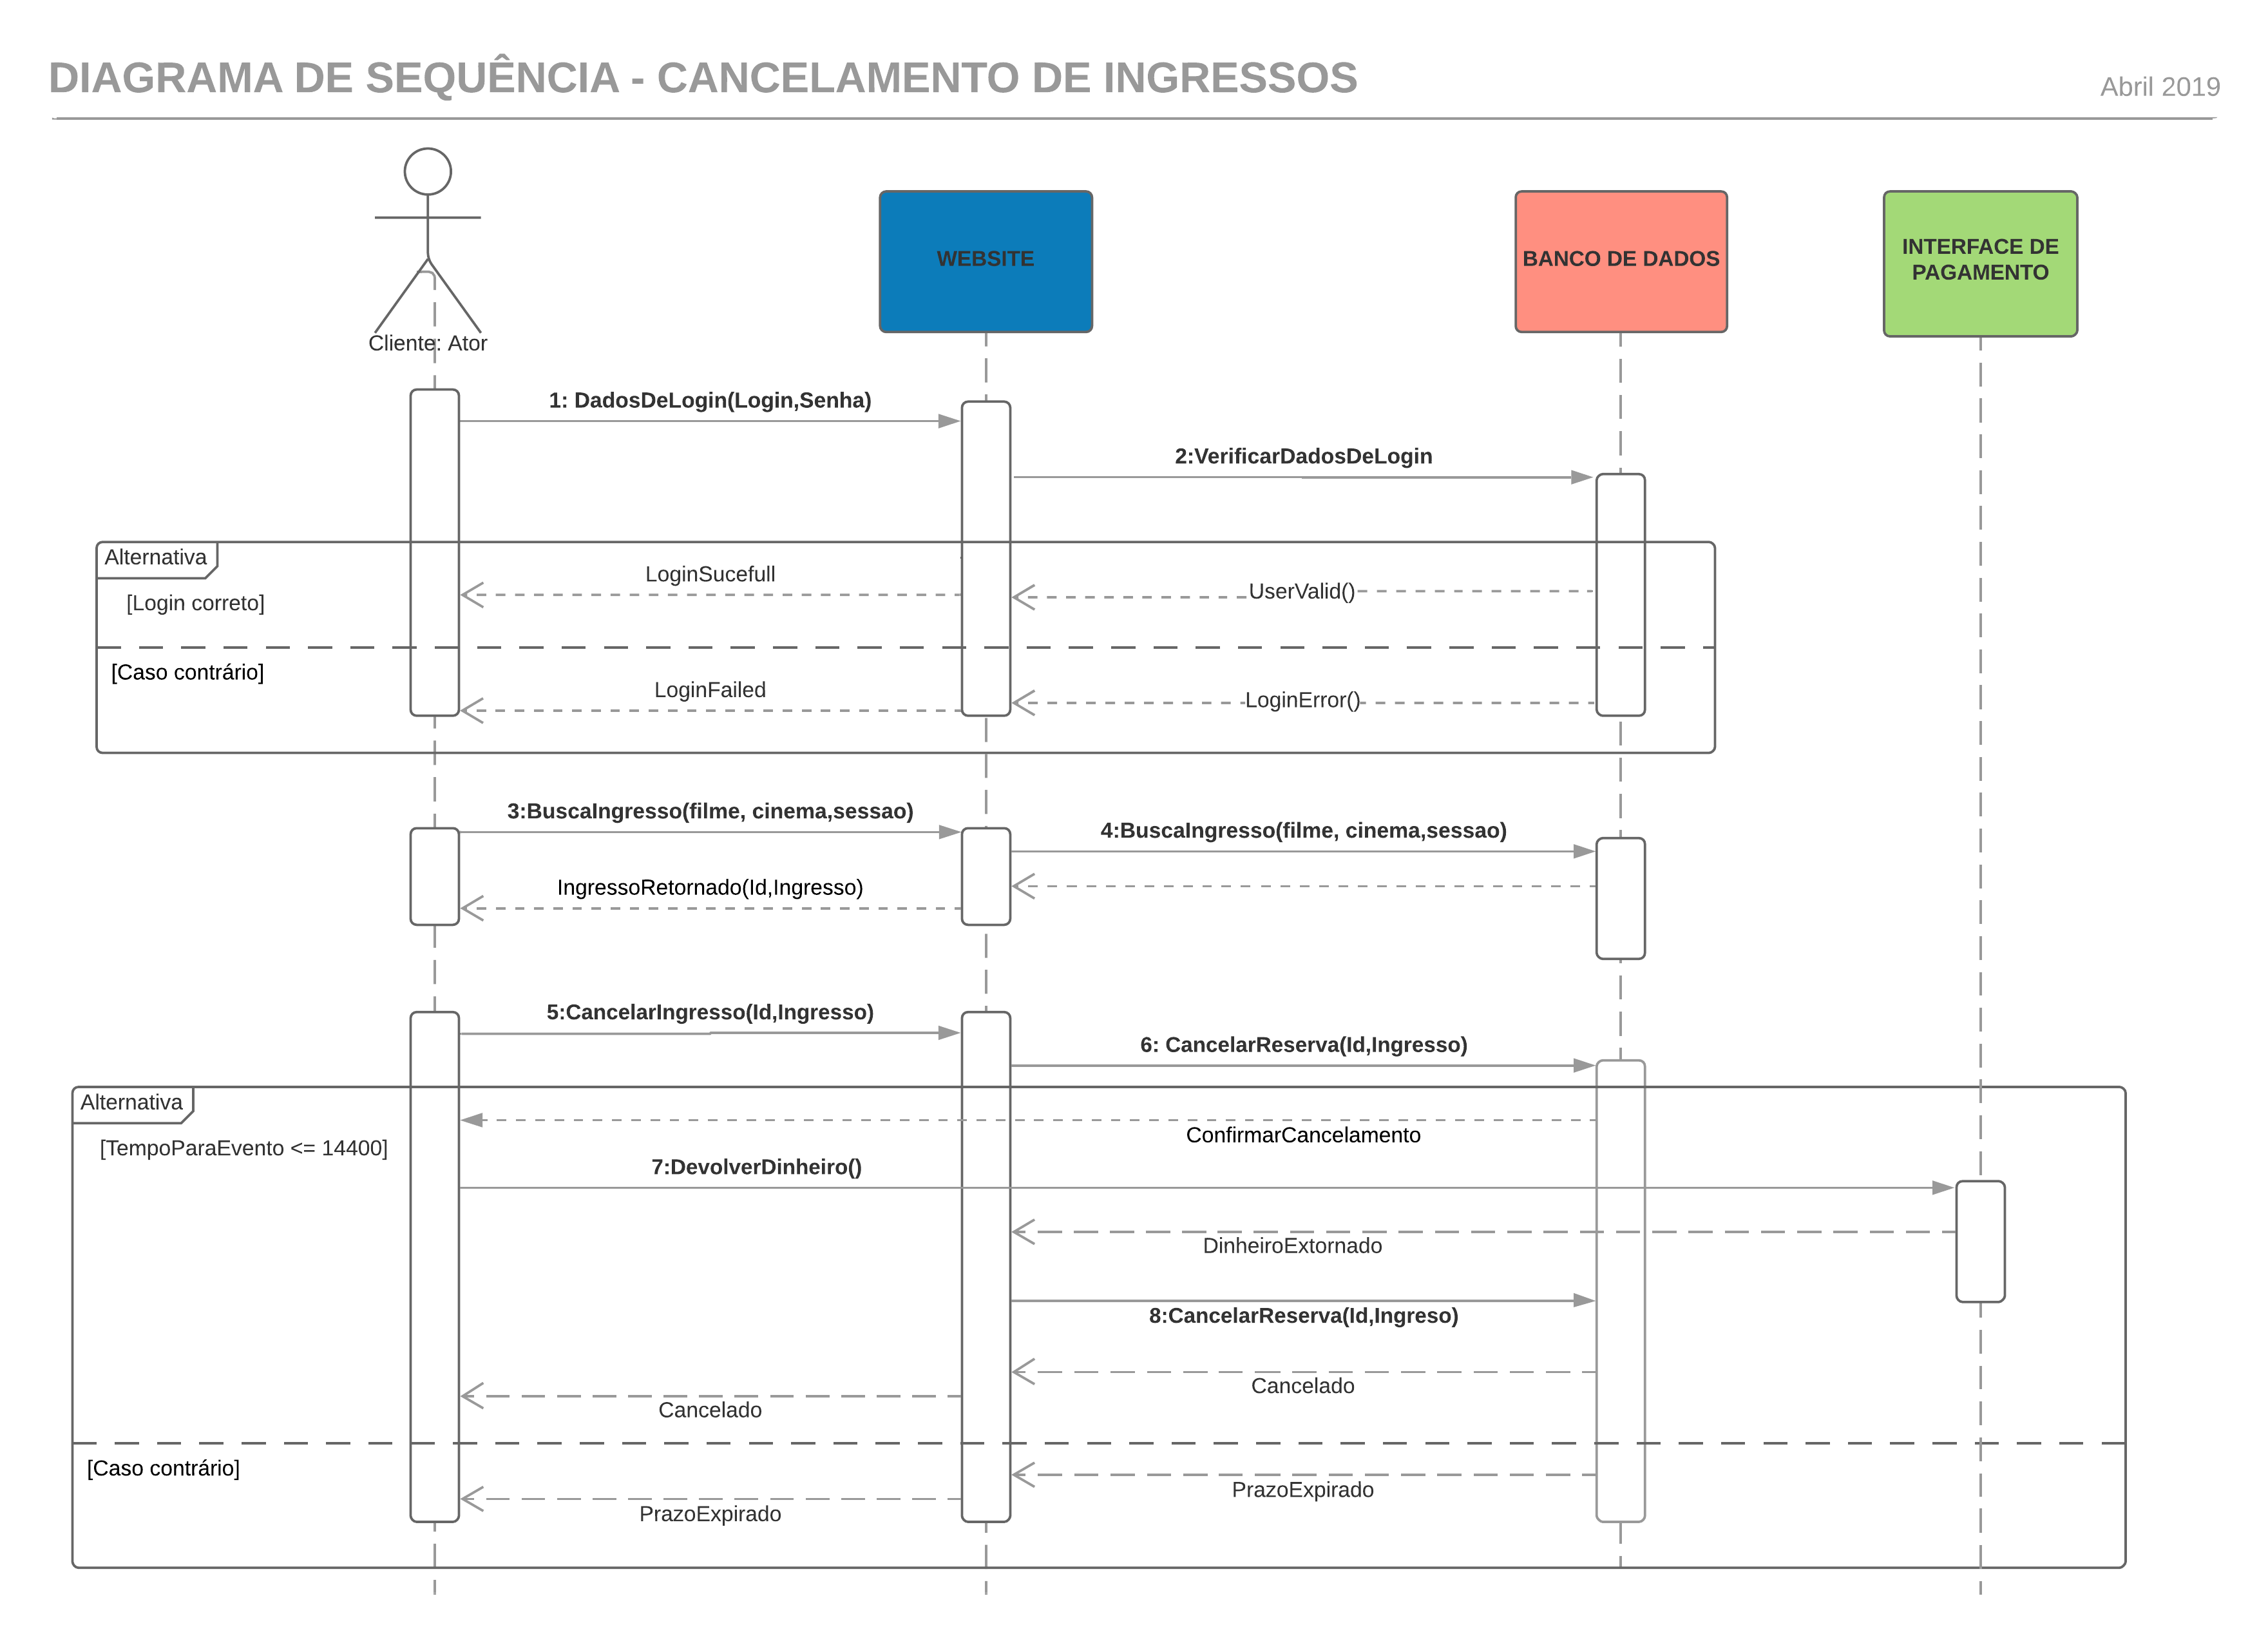
\includegraphics[scale=0.45]{./Imagens/DiagramasDeSequencia/DiagramaDeSequencia3.png}
        \caption{Diagrama de sequencia - Cancelamento de ingressos}
        \label{fig:DiagramaSequencia03}
    \end{figure}

    \begin{figure}[h]
        \centering
        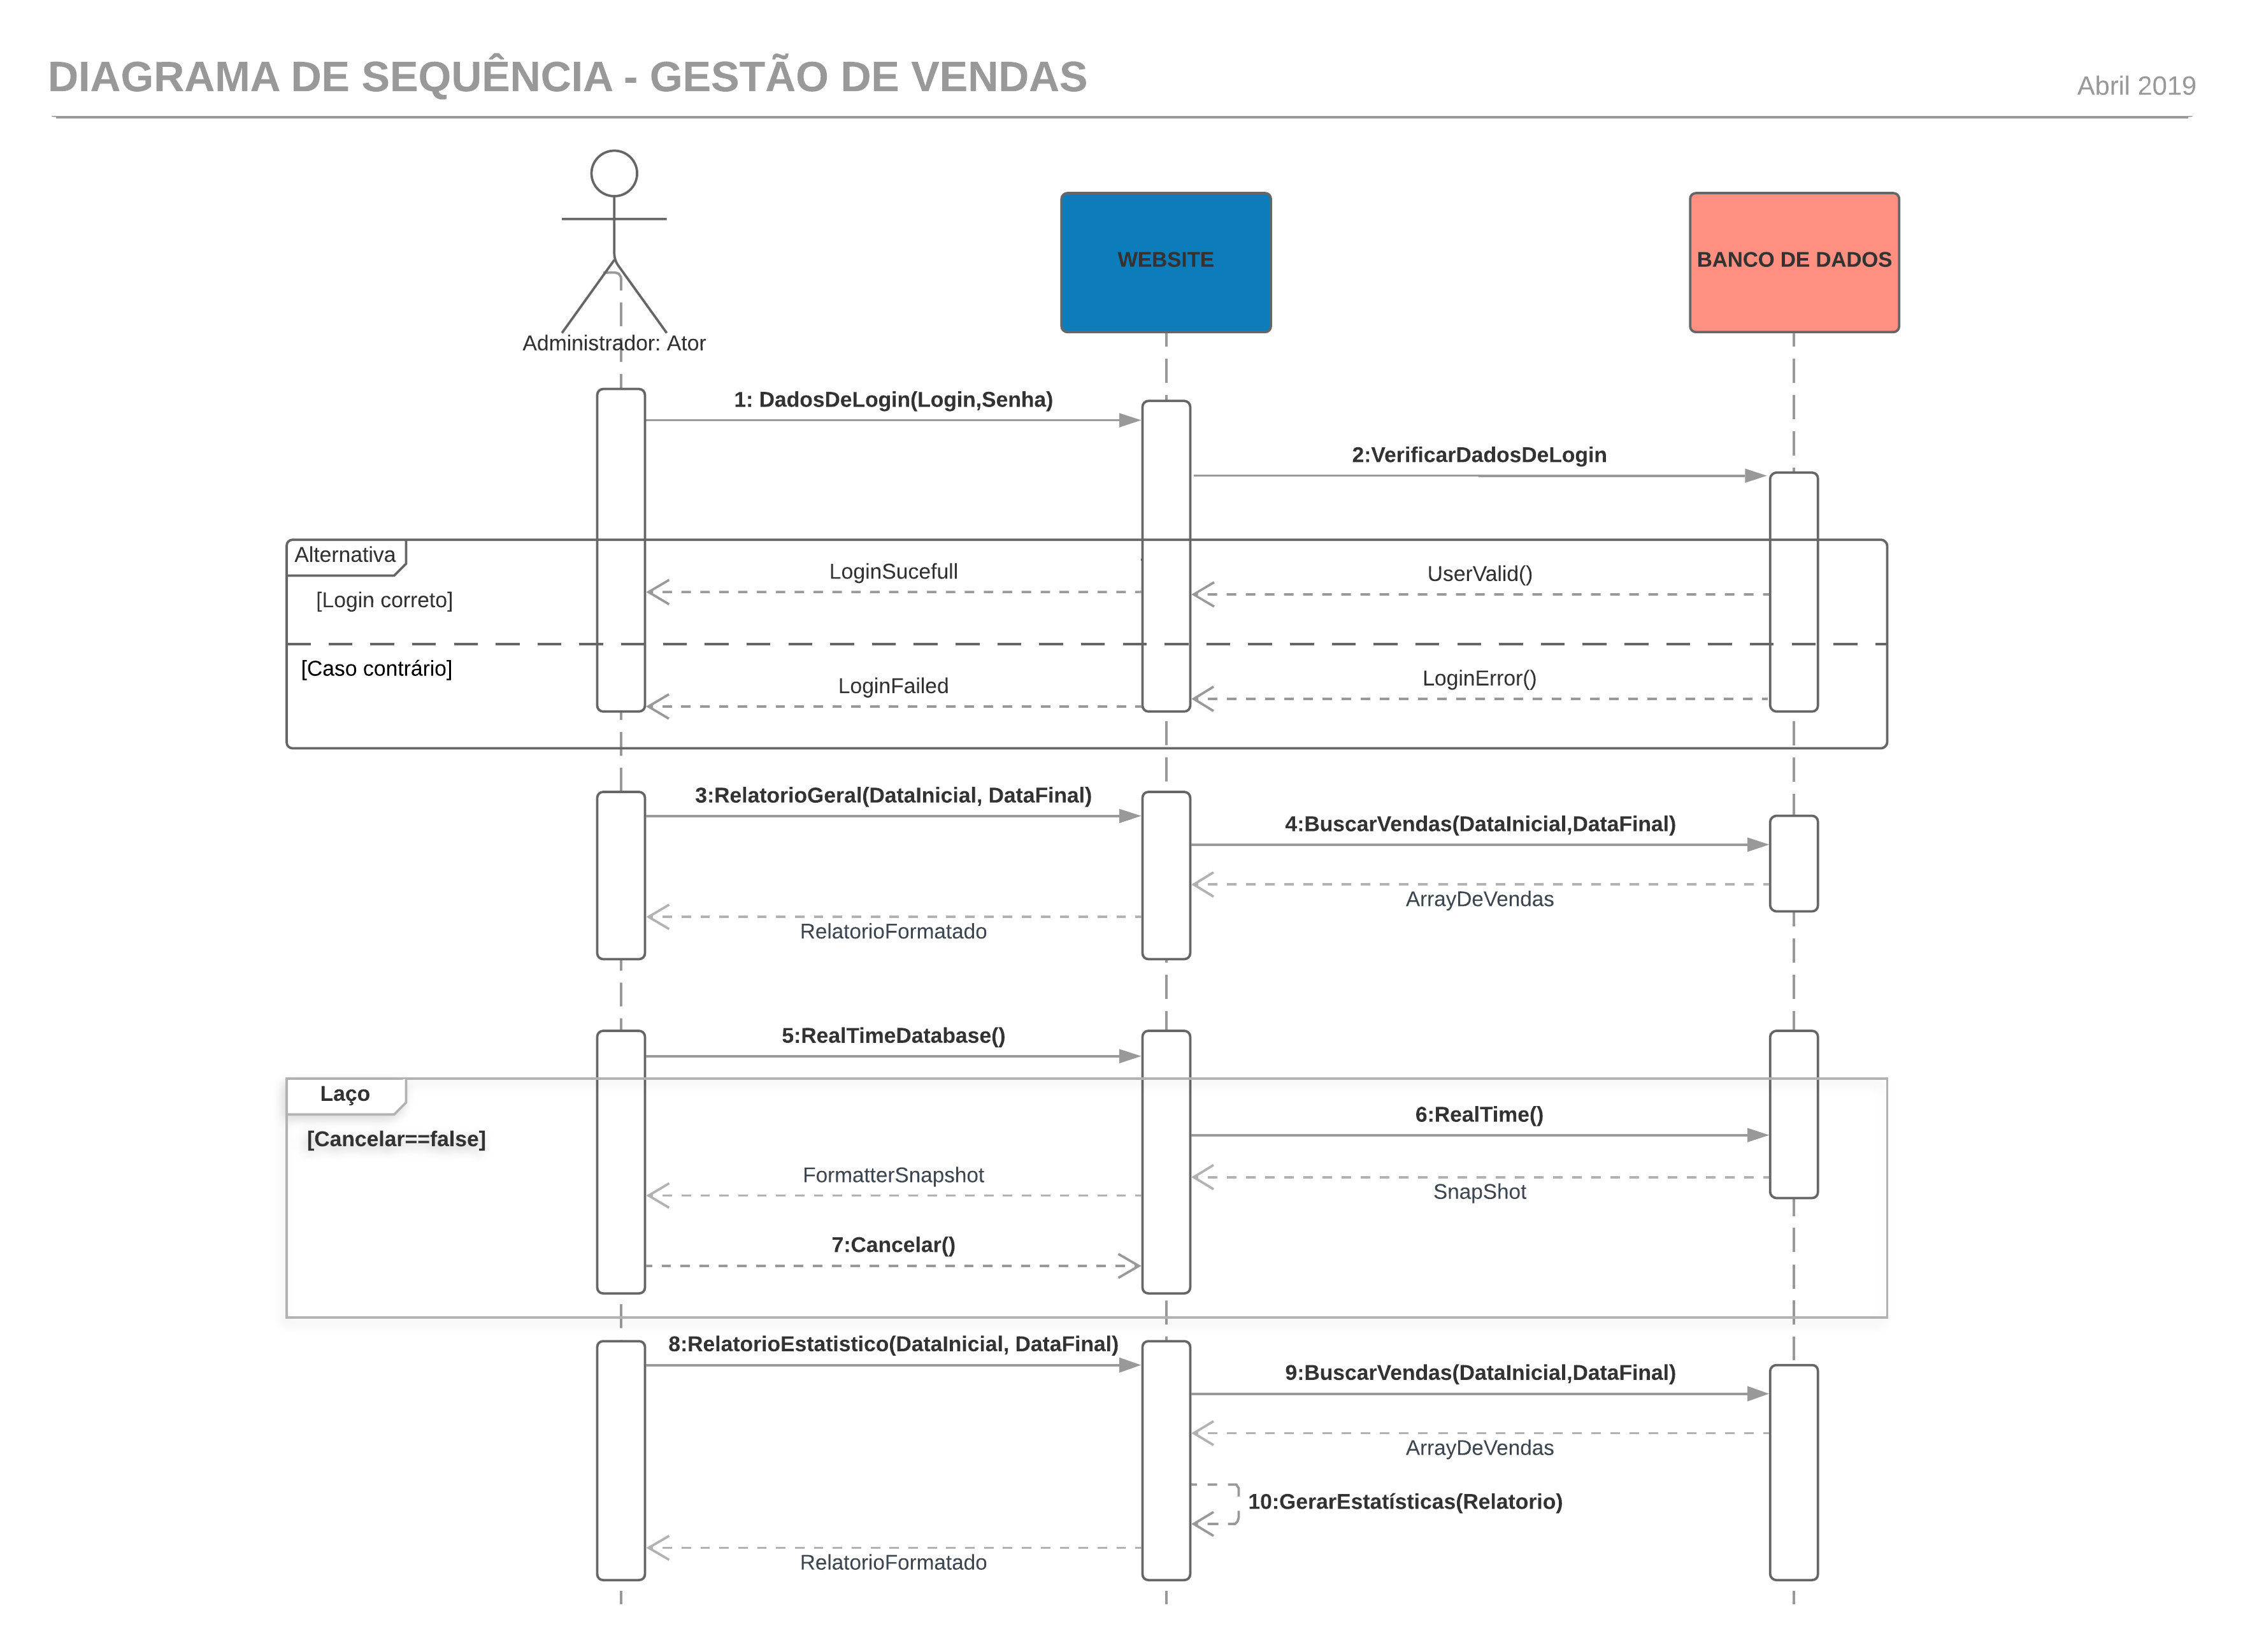
\includegraphics[scale=0.5]{./Imagens/DiagramasDeSequencia/DiagramaDeSequencia4.png}
        \caption{Diagrama de sequencia - Gestão de Vendas}
        \label{fig:DiagramaSequencia04}
    \end{figure}
    \FloatBarrier

    \begin{figure}[h]
        \centering
        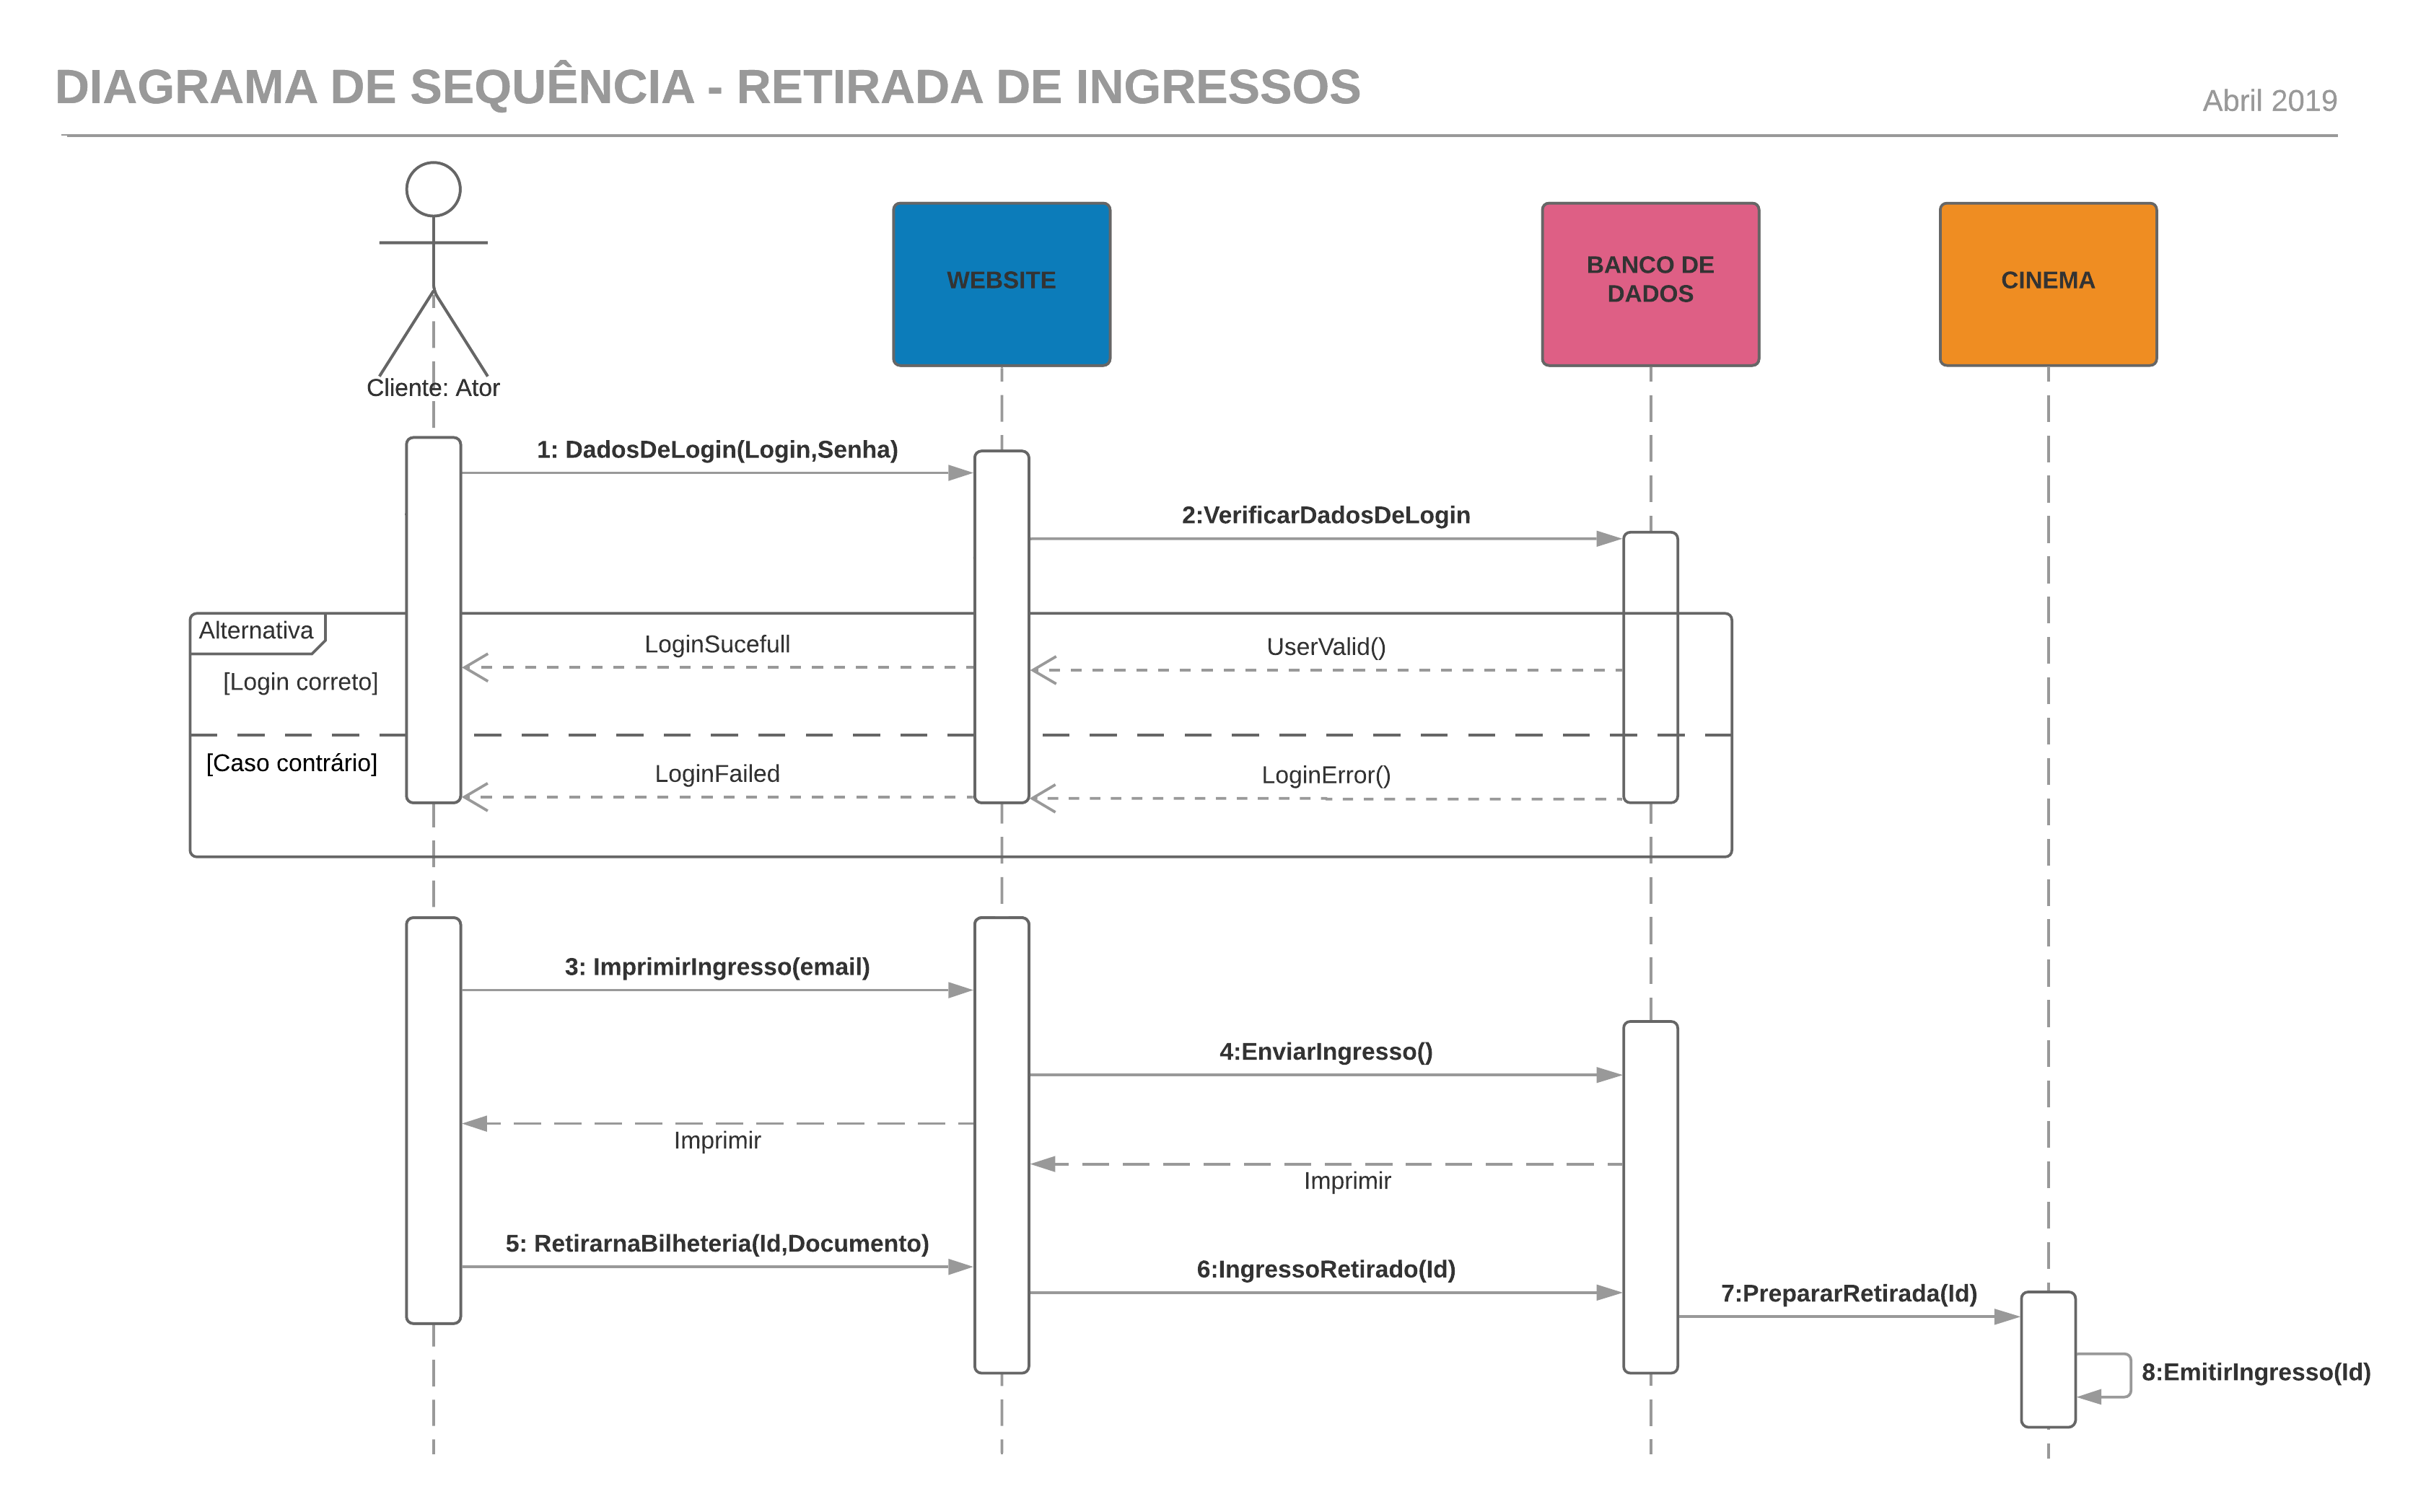
\includegraphics[scale=0.5]{./Imagens/DiagramasDeSequencia/DiagramaDeSequencia5.png}
        \caption{Diagrama de sequencia - Retirada de ingressos}
        \label{fig:DiagramaSequencia05}
    \end{figure}
    \FloatBarrier

    \begin{figure}[h]
        \centering
        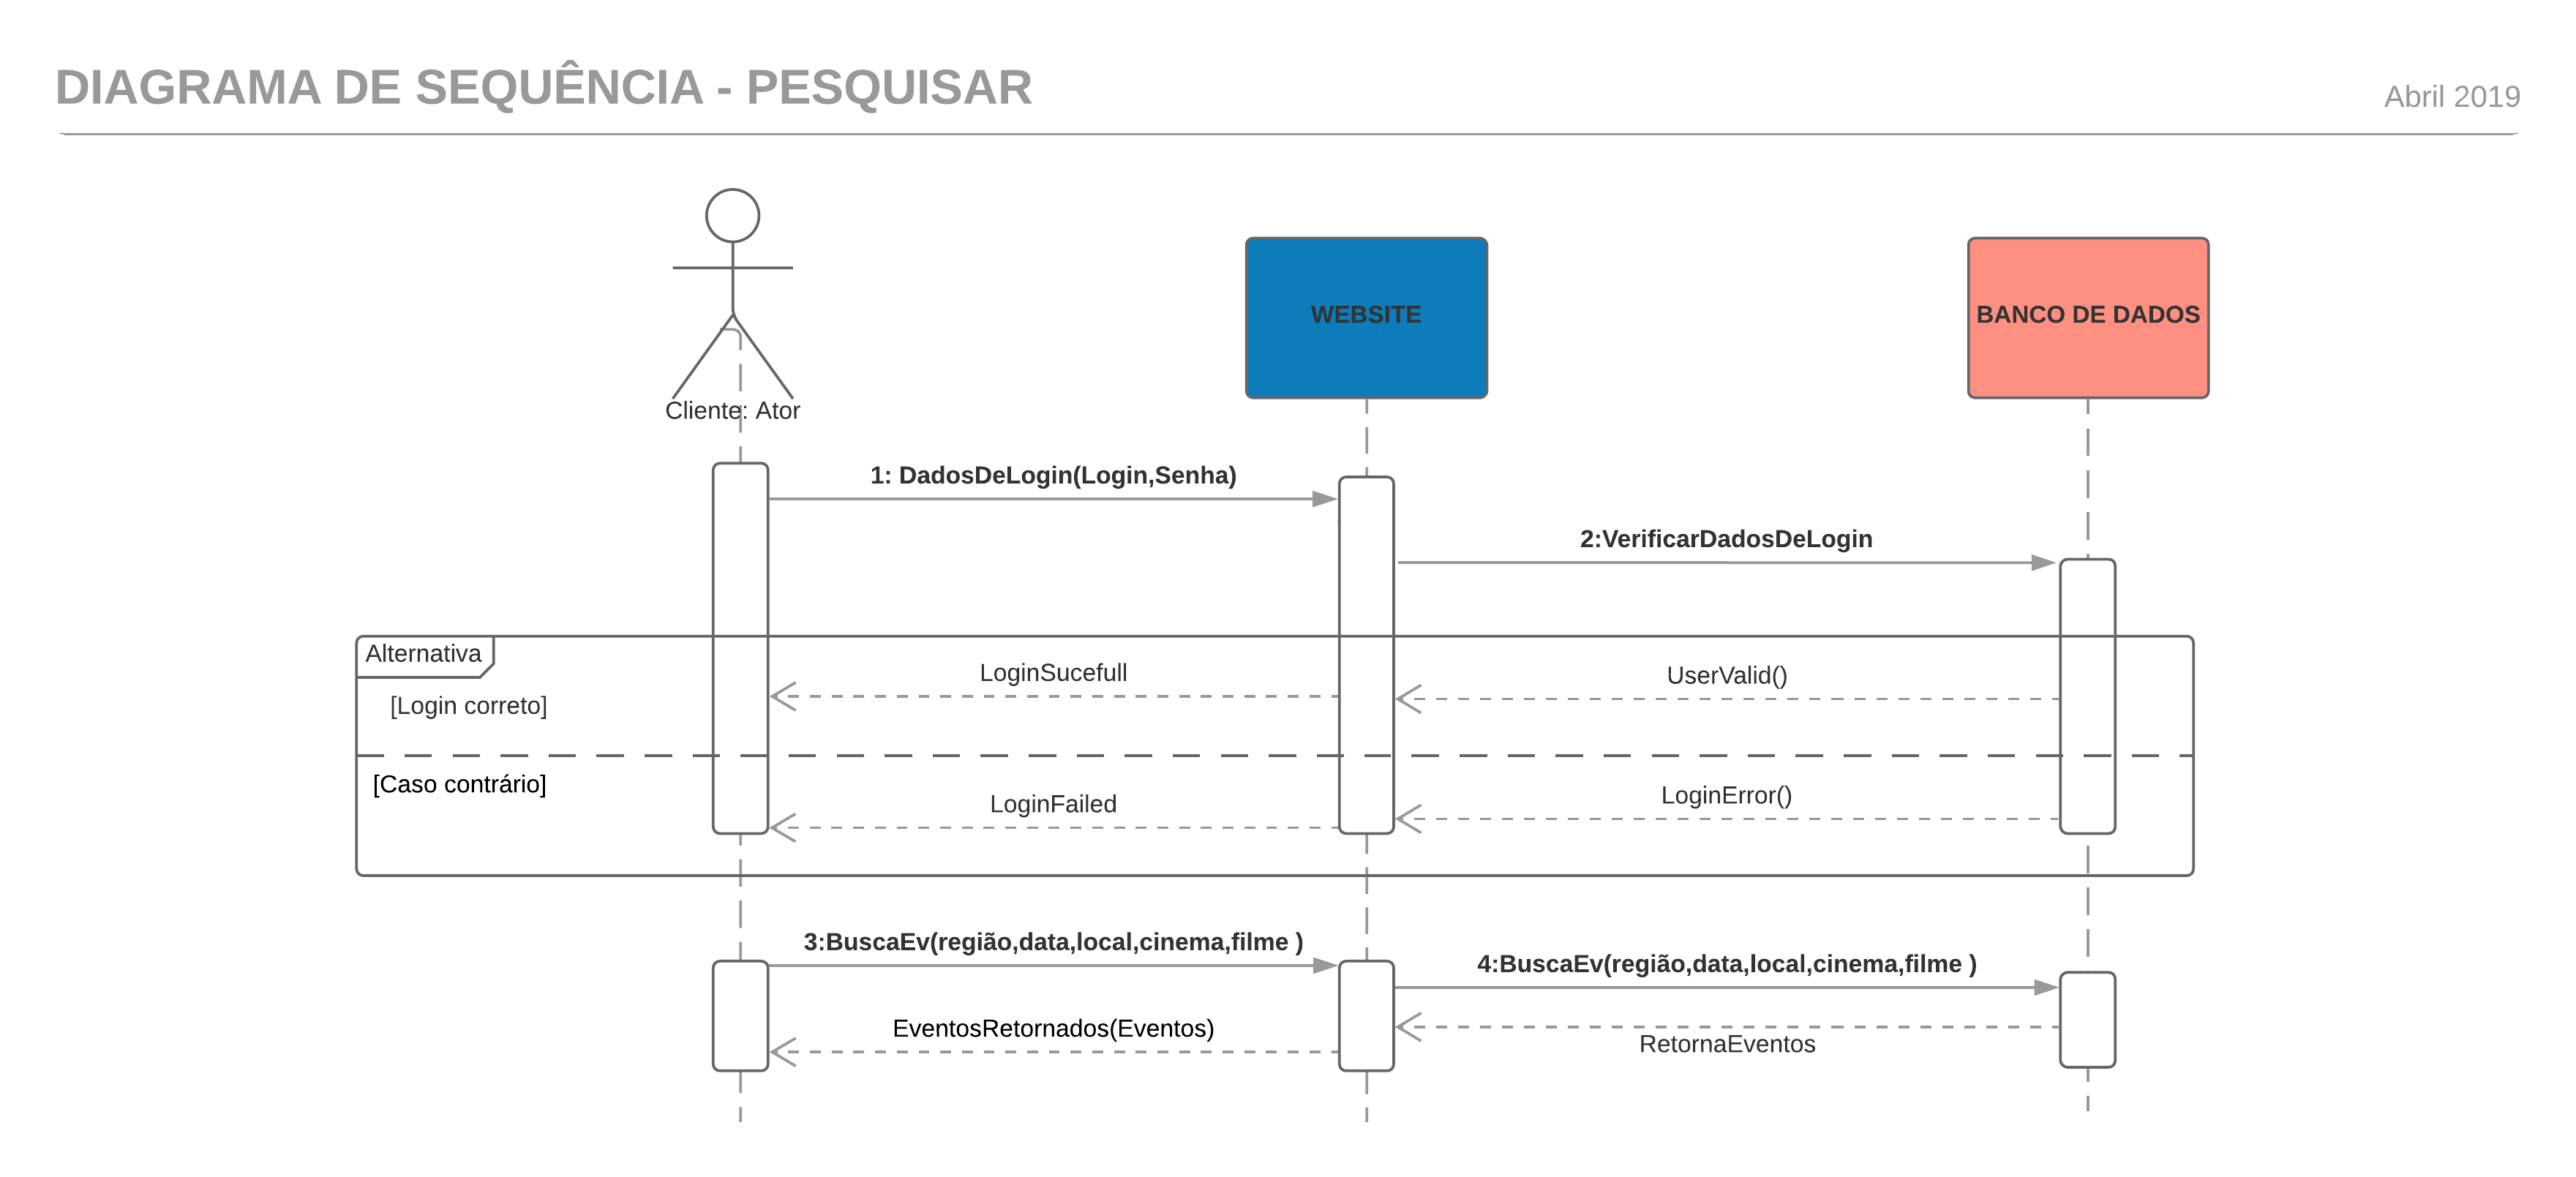
\includegraphics[scale=0.5]{./Imagens/DiagramasDeSequencia/DiagramaDeSequencia6.png}
        \caption{Diagrama de sequencia - Pesquisar}
        \label{fig:DiagramaSequencia06}
    \end{figure}
    \FloatBarrier

    \begin{figure}[h]
        \centering
        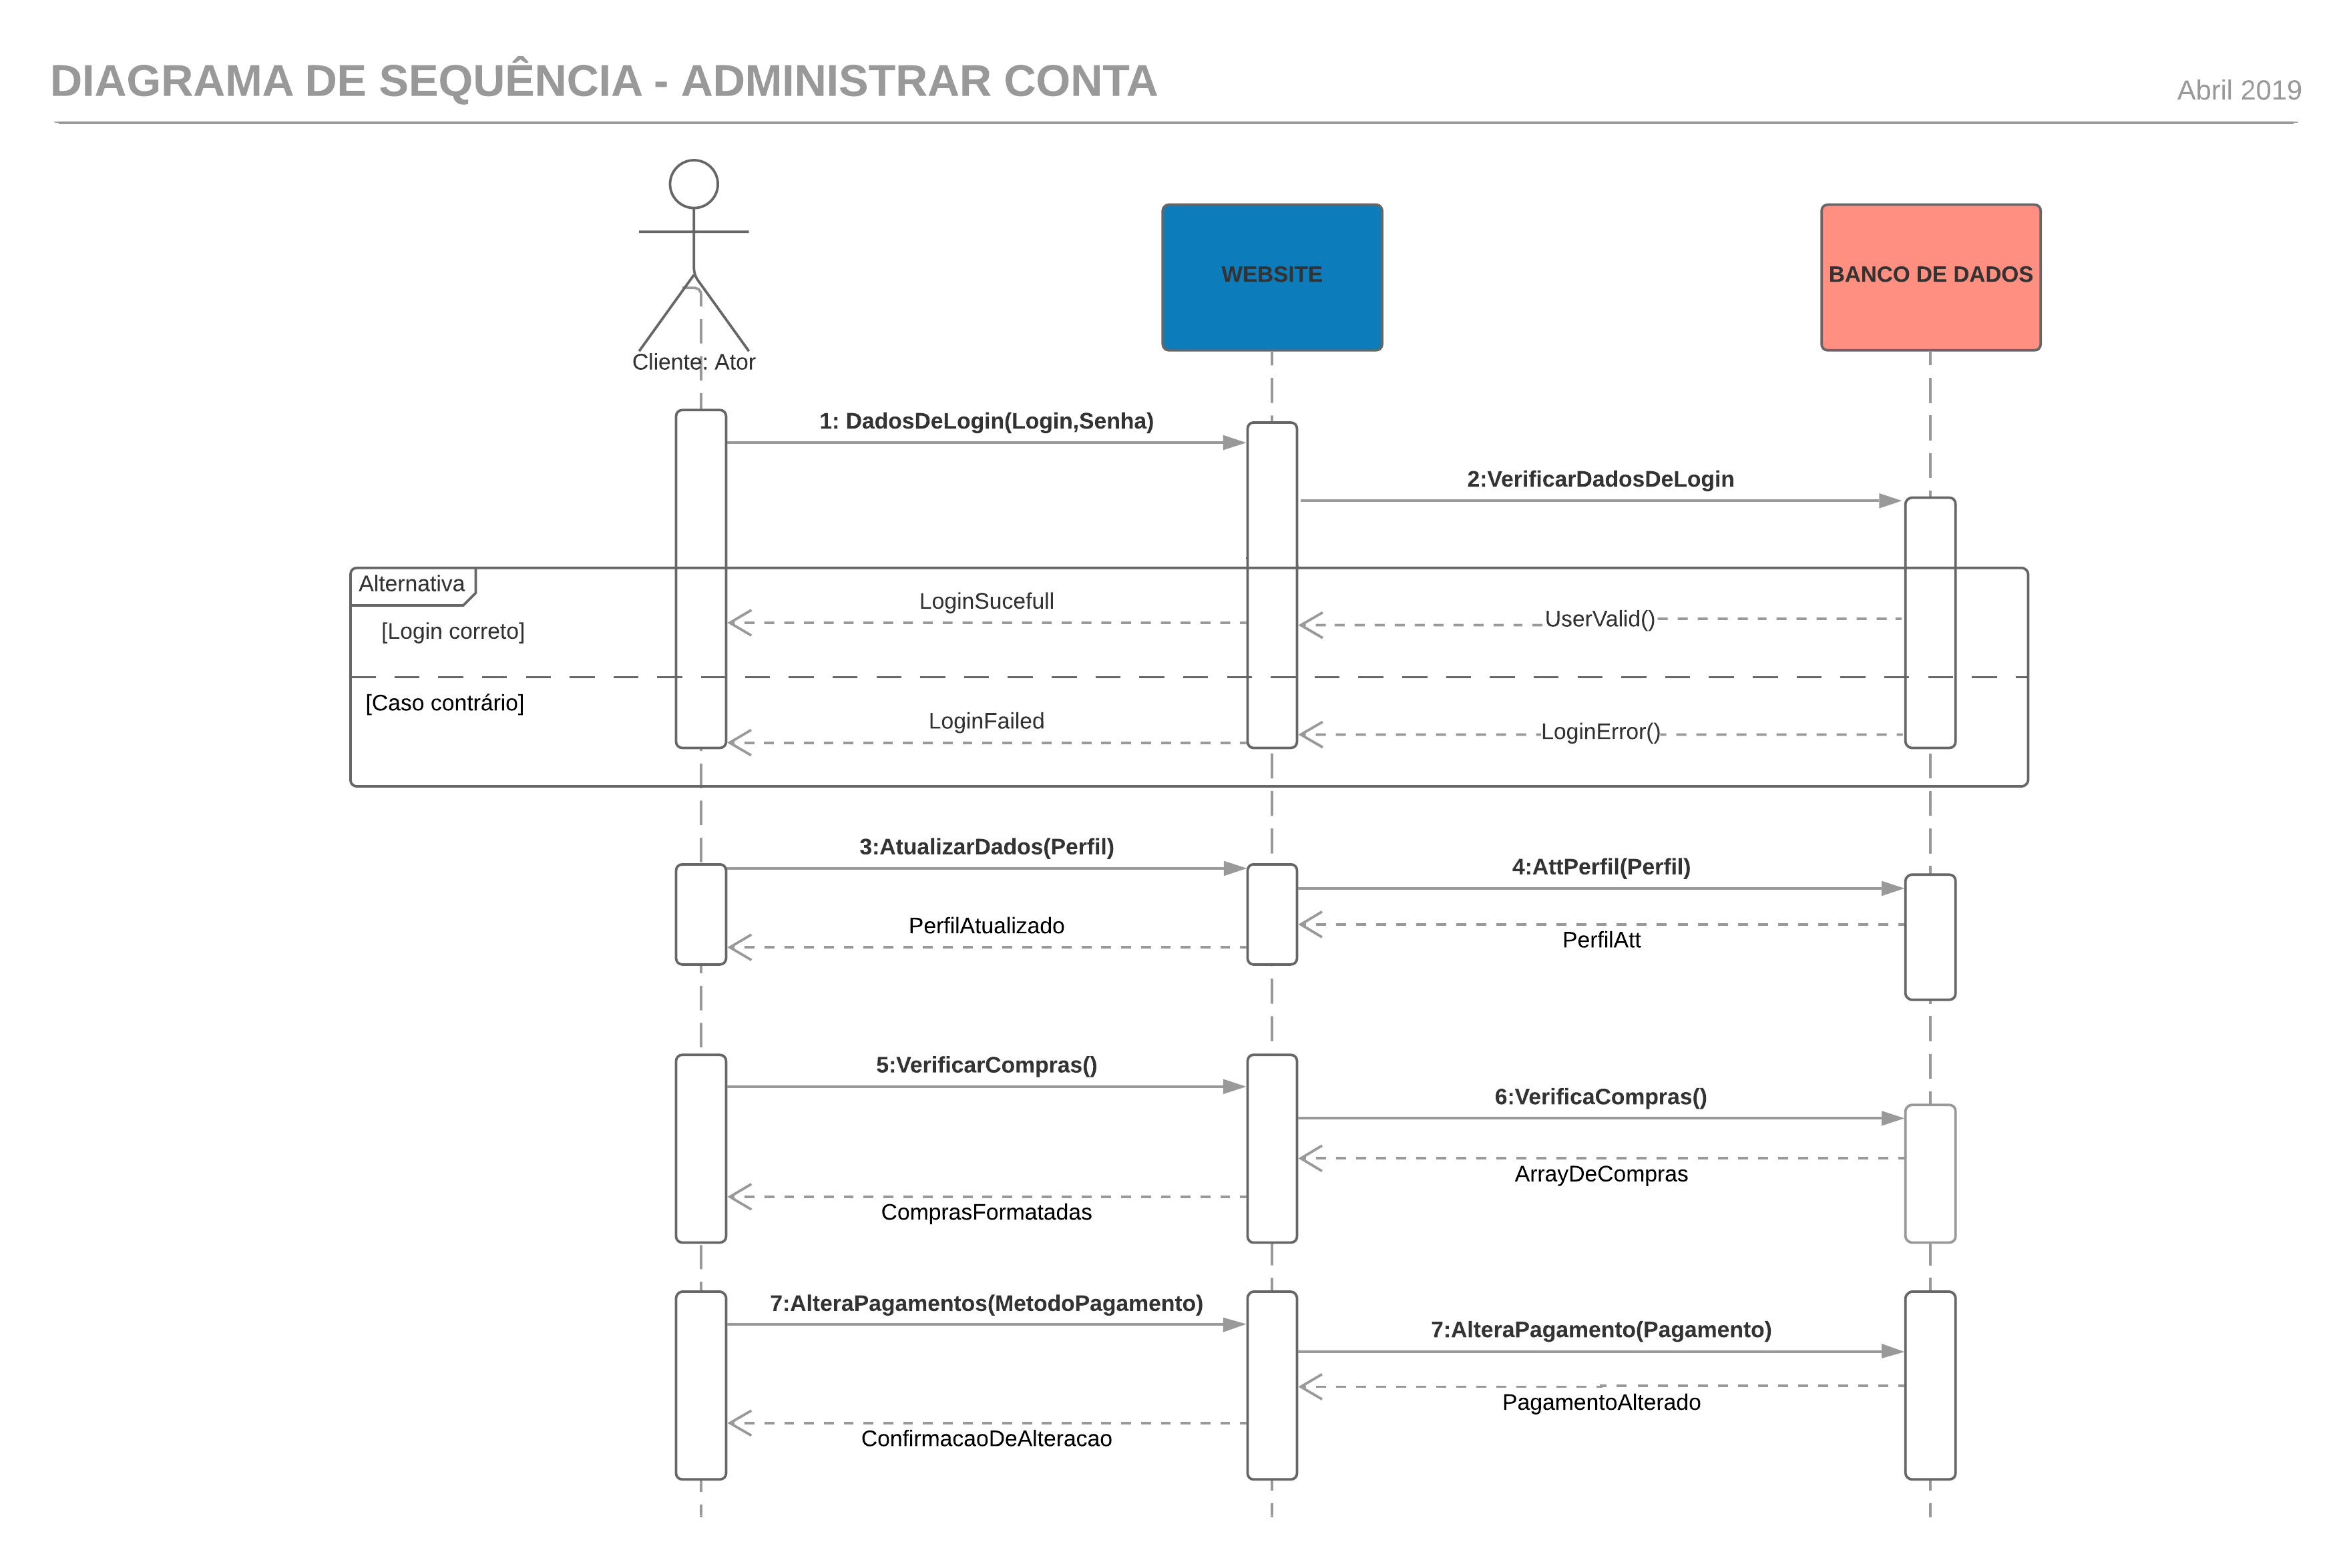
\includegraphics[scale=0.5]{./Imagens/DiagramasDeSequencia/DiagramaDeSequencia7.png}
        \caption{Diagrama de sequencia - Administrar Conta}
        \label{fig:DiagramaSequencia07}
    \end{figure}
    \FloatBarrier
    
    \begin{figure}[h]
        \centering
        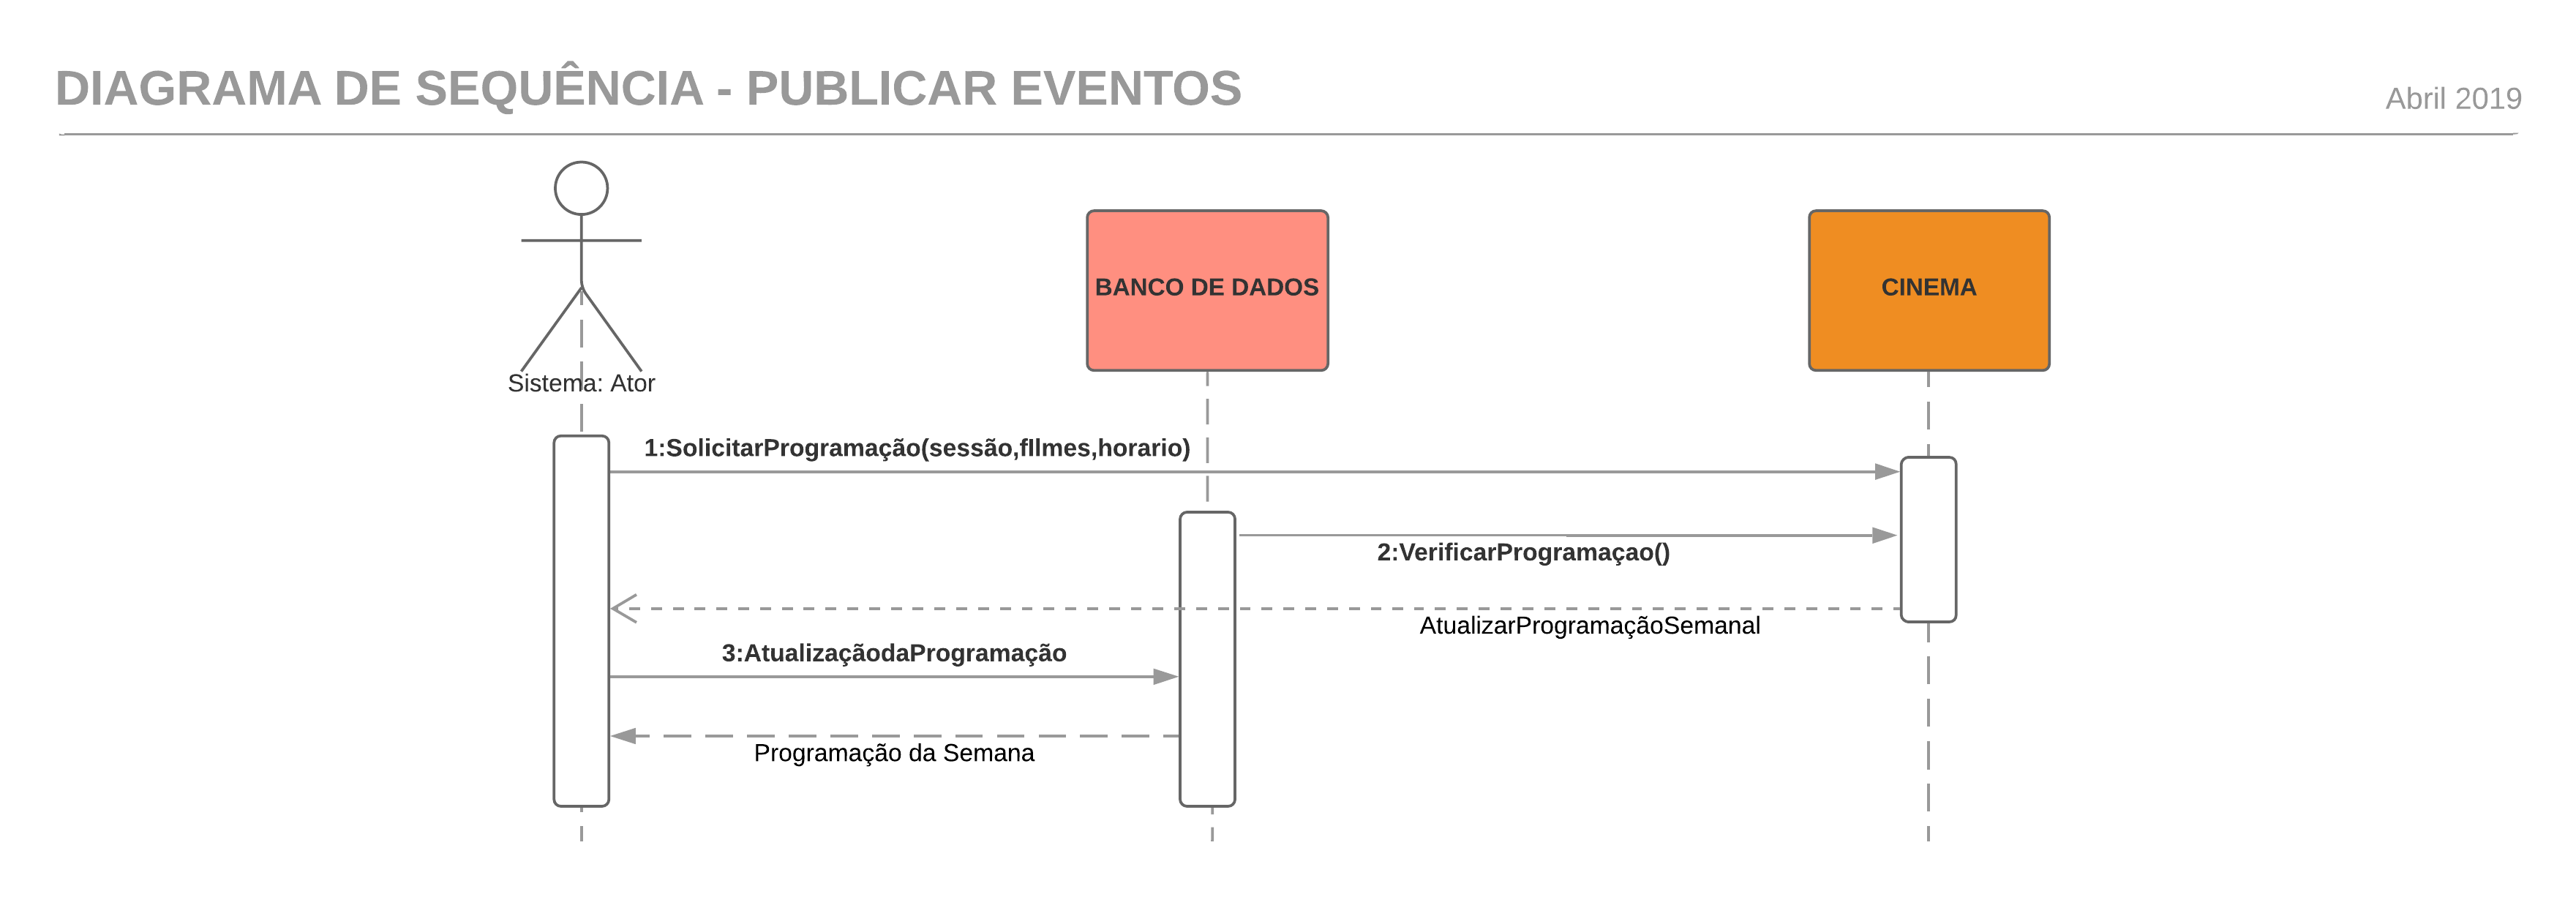
\includegraphics[scale=0.5]{./Imagens/DiagramasDeSequencia/DiagramaDeSequencia8.png}
        \caption{Diagrama de sequencia - Publicar Eventos}
        \label{fig:DiagramaSequencia08}
    \end{figure}
    \FloatBarrier
    
    \begin{figure}[h]
        \centering
        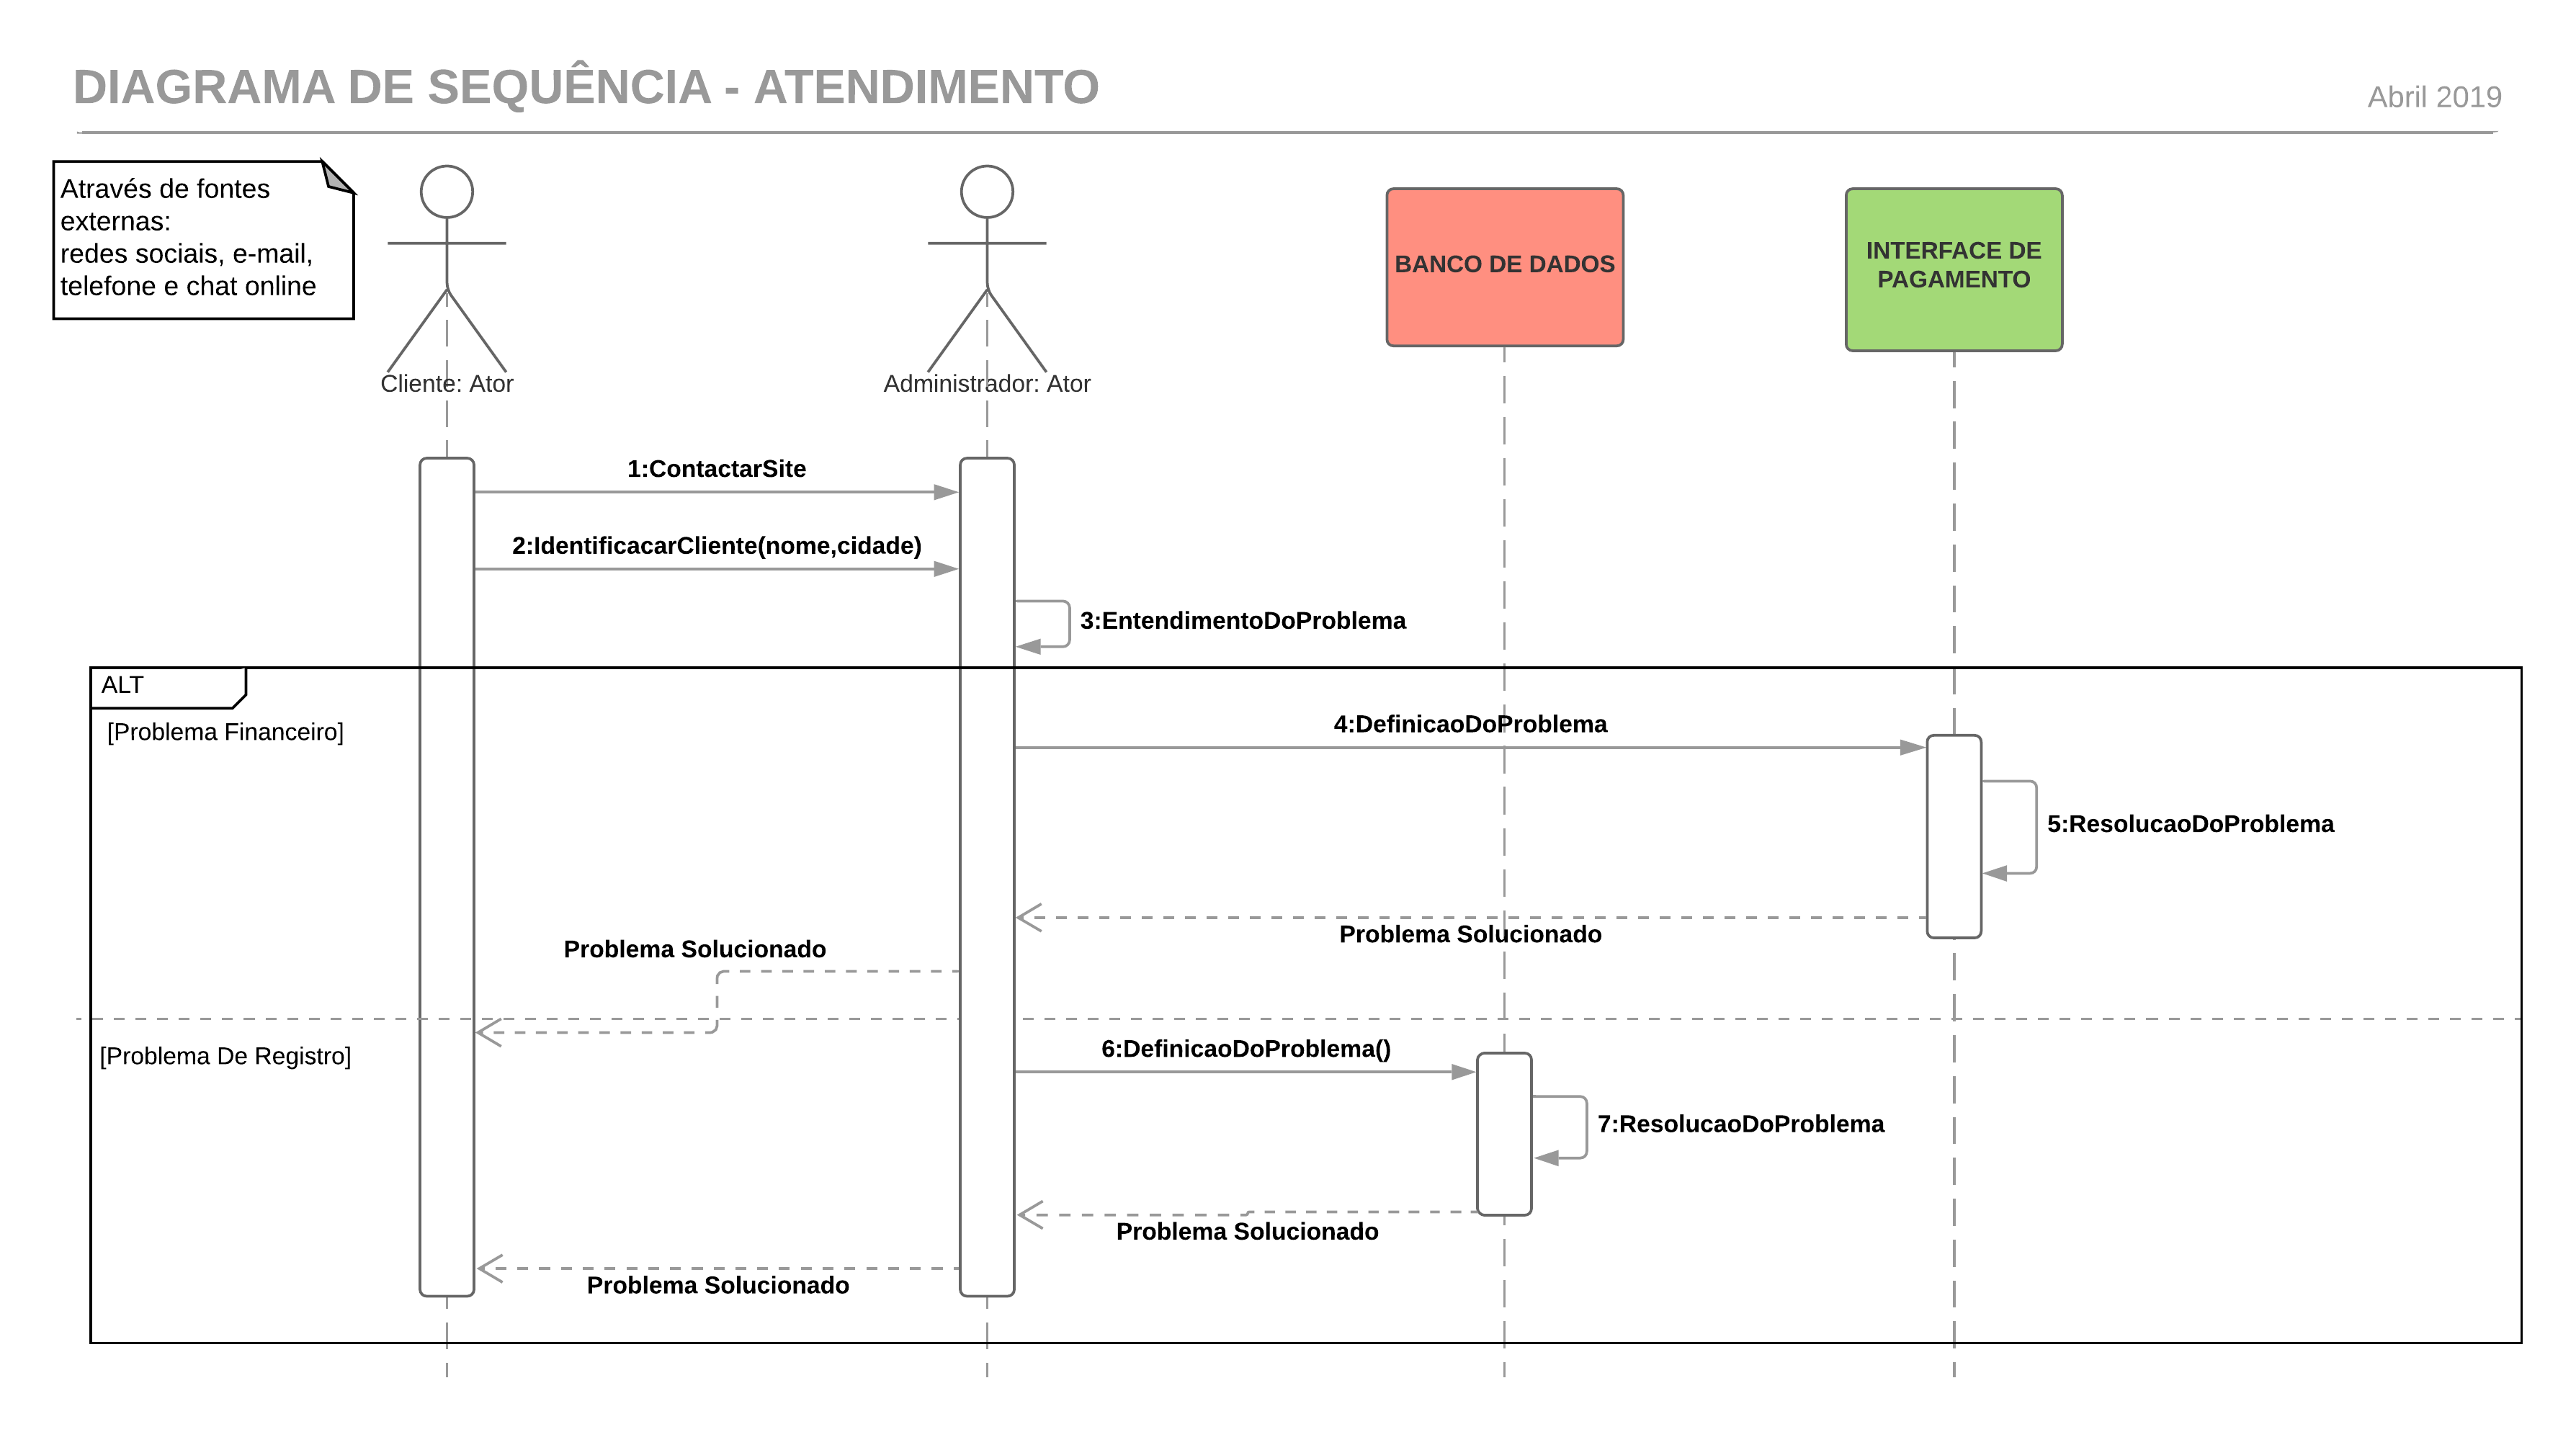
\includegraphics[scale=0.5]{./Imagens/DiagramasDeSequencia/DiagramaDeSequencia9.png}
        \caption{Diagrama de sequencia - Atendimento}
        \label{fig:DiagramaSequencia09}
    \end{figure}
    \FloatBarrier

\section{Necessidades de Usuários}
    \subsection{WebSites para compra de ingressos}
        WebSites oferece ao consumidor simplicidade, agilidade e comodidade na hora de comprar um ingresso (sem demora e sem filas), então analisamos o funcionamento de alguns WebSites de vendas de ingresso de cinema.

	    Foi feita uma pesquisa no Google onde encontramos sites de venda, o primeiro site escolhido foi o que apareceu em primeiro lugar em forma de publicidade: \cite{letsEvents}.
	
	    Se chama Lets.events, nele além de comprar ingressos, você pode também criar eventos para vender seus ingressos. A primeira vista é um site receptivo com imagens coloridas e bastante informação de como comprar incluindo valores de taxas que você irá pagar na compra, junto do valor da taxa há um especificação de que naquela site você encontra as menores taxas do mercado. 
        No site também há uma plataforma de atendimento a pessoa que deseja criar eventos.
        Quando se clica em encontrar eventos, logo carrega uma página com eventos recentes e campo para procura do que você deseja. Digitei cinema e foi retornado, apenas um evento, logo podemos notar que não se trata de cinema em si (com salas e telas), mas sim eventos culturais que acontecem em locais diferentes e até mesmo ao ar livre. 
        Ponto positivo é que há toda uma especificação do local, horário, valores, organizadores, enfim, bem completo. Na hora da compra você escolhe a quantidade de ingressos e se é meia entrada com promoção, insere seus dados e realiza a compra. Para finalizar é apenas imprimir seu ingresso.

        Na segunda pesquisa parece que houve um erro no site que logo mais explicarei sobre. O segundo site estava entre as pesquisas do topo, se trata do site \cite{Cinemark}. É um site do próprio cinema, sua apresentação é simples e sem muitos detalhes chamativos, mas contém todas as informações necessárias. Uma elemento que chamou a atenção foi a venda de ingressos corporativos que fornece uma promoção para aqueles que querem presentear a equipe de funcionários de uma empresa com uma sessão de cinema que acompanha um brinde. Isso é uma forma atrativa e criativa de venda de ingressos, possibilitando assim que mais pessoas tenham acesso ao cinema. Como dito anteriormente, quando acessado o E-COMMERCE para a compra de ingressos corporativos teve uma uma demora de aproximadamente 15 minutos para que carregasse a página, o que é um ponto negativo para o site.
        Na busca por ingressos, há uma apresentação dos shoppings que possuem o Cinemark, para que o cliente possa escolher a melhor localização, há também a busca por ingressos do filme que você deseja assistir. 
        Os filmes disponíveis estão em programação, lá você pode escolher horários, filmes e localização. Ponto positivo é que há cardápio de lanchonete do cinema e também promoções de ingressos para clientes assíduos.
        É um site completo que com certeza nos ajudaria na compra de ingressos.

	    Terceiro site visitado é um bem comum \cite{ingresso.com}, abrange muitos estados do Brasil, onde você pode escolher sua localização. Na página inicial já aparece todos os filmes em cartaz e o mais procurado é evidenciado no topo.
	    Tem a opção de escolha de filmes, cinema e eventos para compra de ingressos, conta também com atendimento ao consumidor.
	    Ao clicar no filme desejado aparece todos os cinemas na cidade escolhida, bem como os horários de transmissão e em qual horário possui o filme, em 3D se é dublado ou legendado e a sala dos filmes, possuindo também o guia de salas.Na hora da compra você escolhe as poltronas disponíveis e poltronas especiais, o que é um ponto positivo na organização de um lugar e se deseja adicionar pipoca ao valor do ingresso na hora de pagar. 
	    Finalizando você escolhe a forma de pagamento e imprime seu ingresso. Por fim, notamos que é um site completo e útil que com certeza iremos recomendar.
	
	\subsection{Experiências de familiares e amigos sobre compra de ingresso de cinema }
	    Melhor maneira encontrada de lidar e organizar pesquisas foi criando um questionário objetivo, pois é rápido e eficaz. Foram entrevistadas 11 pessoas, tanto parentes como amigos próximos com intuito de sabermos suas experiências, preferências e até mesmo o que para eles seriam importante na hora da compra de um ingresso de cinema.
        Será apresentado agora tabelas com os dados coletados.

        \begin{table}[h]
            \centering
            \resizebox{\textwidth}{!}{
                \begin{tabular}{|c|c|c|c|c|c|c|c|c|c|c|c|}
                    \hline
                    \multicolumn{1}{|c|}{\textbf{}} & 
                    \multicolumn{1}{c|}{\textbf{Carlos}} & 
                    \multicolumn{1}{c|}{\textbf{Danilo}} & 
                    \multicolumn{1}{c|}{\textbf{Gabriel}} & 
                    \multicolumn{1}{c|}{\textbf{Giovani}} & 
                    \multicolumn{1}{c|}{\textbf{Giovanna}} & 
                    \multicolumn{1}{c|}{\textbf{Guilherme}} & 
                    \multicolumn{1}{c|}{\textbf{Indianara}} &
                    \multicolumn{1}{c|}{\textbf{Luiz}} &
                    \multicolumn{1}{c|}{\textbf{Micael}} &
                    \multicolumn{1}{c|}{\textbf{Nicole}} &
                    \multicolumn{1}{c|}{\textbf{Vanessa}} \\ \hline
                    Em casa & & X & & & & & X & & X & X & X \\ \hline
                    No cinema & & & X & X & X & X & & X & & & \\ \hline
                \end{tabular}
            }
            \caption{Preferência de local para ver filme}
            \label{table:preferencia_local_ver_filme}
        \end{table}
        \FloatBarrier
    
        Na Tabela \ref{table:preferencia_local_ver_filme} podemos notar que maioria dos entrevistados preferem ver um filme no cinema, mas a disputa ficou em acirrada entre os que preferem o conforto de casa ou invés da descontração e tela gigante do cinema.

        \begin{table}[h]
            \centering
            \resizebox{\textwidth}{!}{
                \begin{tabular}{|c|c|c|c|c|c|c|c|c|c|c|c|c|}
                    \hline
                    \multicolumn{1}{|c|}{\textbf{}} & 
                    \multicolumn{1}{c|}{\textbf{Carlos}} & 
                    \multicolumn{1}{c|}{\textbf{Danilo}} & 
                    \multicolumn{1}{c|}{\textbf{Gabriel}} & 
                    \multicolumn{1}{c|}{\textbf{Giovani}} & 
                    \multicolumn{1}{c|}{\textbf{Giovanna}} & 
                    \multicolumn{1}{c|}{\textbf{Guilherme}} & 
                    \multicolumn{1}{c|}{\textbf{Indianara}} &
                    \multicolumn{1}{c|}{\textbf{Luiz}} &
                    \multicolumn{1}{c|}{\textbf{Micael}} &
                    \multicolumn{1}{c|}{\textbf{Nicole}} &
                    \multicolumn{1}{c|}{\textbf{Vanessa}} &
                    \multicolumn{1}{c|}{\textbf{Média}}\\ \hline
                    Alimentação Disponível & 5 & 10 & 3 & 1 & 0 & 6 & 5 & 6 & 10 & 5 & 8 & 5.4\\ \hline
                    Preço do ingresso & 8 & 9 & 8 & 10 & 10 & 8 & 10 & 9 & 10 & 10 & 10 & 9.2\\ \hline
                    Localização & 8 & 5 & 5 & 6 & 10 & 6 & 5 & 6 & 10 & 8 & 7 & 6.9\\ \hline
                    Ambiente confortável  & 9 & 7 & 8 & 7 & 9 & 9 & 9 & 6 & 10 & 9 & 9 & 8.3\\ \hline
                    Disponibilidade de horário  & 9 & 4 & 8 & 8 & 7 & 9 & 8 & 9 & 10 & 10 & 8 & 8.1\\ \hline
                \end{tabular}
            }
            \caption{Representação de 1 a 10 na hora de escolher um cinema}
            \label{table:esolha_de_cinema}
        \end{table}
        \FloatBarrier
        Feito a média de cada tópico levantado na Tabela \ref{table:esolha_de_cinema}, ficou claro que a maioria dos entrevistados estão mesmo preocupados mais com o preço do ingresso na hora de adquirir um e que não importa muito para alguns que haja comida no estabelecimento.

        \begin{table}[h]
            \centering
            \resizebox{\textwidth}{!}{
                \begin{tabular}{|c|c|c|c|c|c|c|c|c|c|c|c|}
                    \hline
                    \multicolumn{1}{|c|}{\textbf{}} & 
                    \multicolumn{1}{c|}{\textbf{Carlos}} & 
                    \multicolumn{1}{c|}{\textbf{Danilo}} & 
                    \multicolumn{1}{c|}{\textbf{Gabriel}} & 
                    \multicolumn{1}{c|}{\textbf{Giovani}} & 
                    \multicolumn{1}{c|}{\textbf{Giovanna}} & 
                    \multicolumn{1}{c|}{\textbf{Guilherme}} & 
                    \multicolumn{1}{c|}{\textbf{Indianara}} &
                    \multicolumn{1}{c|}{\textbf{Luiz}} &
                    \multicolumn{1}{c|}{\textbf{Micael}} &
                    \multicolumn{1}{c|}{\textbf{Nicole}} &
                    \multicolumn{1}{c|}{\textbf{Vanessa}} \\ \hline
                    Aplicativos & & & & & & & & & & & \\ \hline
                    Sites & & & & & & X & & & & X & \\ \hline
                    Presencial & X & X & X & X & X & & X & X & X & & X\\ \hline
                \end{tabular}
            }
            \caption{Meio mais frequente de compra de ingresso}
            \label{table:meio_freq_comp_de_ingresso}
        \end{table}
        \FloatBarrier
        Vendas de ingresso em sites e por aplicativos perdem para a presencial, isso é um ponto que deve ser abordado de como melhorar as vendas já que é mais cômodo comprar pela internet.

        \begin{table}[h]
            \centering
            \resizebox{\textwidth}{!}{
                \begin{tabular}{|c|c|c|c|c|c|c|c|c|c|c|c|}
                    \hline
                    \multicolumn{1}{|c|}{\textbf{}} & 
                    \multicolumn{1}{c|}{\textbf{Carlos}} & 
                    \multicolumn{1}{c|}{\textbf{Danilo}} & 
                    \multicolumn{1}{c|}{\textbf{Gabriel}} & 
                    \multicolumn{1}{c|}{\textbf{Giovani}} & 
                    \multicolumn{1}{c|}{\textbf{Giovanna}} & 
                    \multicolumn{1}{c|}{\textbf{Guilherme}} & 
                    \multicolumn{1}{c|}{\textbf{Indianara}} &
                    \multicolumn{1}{c|}{\textbf{Luiz}} &
                    \multicolumn{1}{c|}{\textbf{Micael}} &
                    \multicolumn{1}{c|}{\textbf{Nicole}} &
                    \multicolumn{1}{c|}{\textbf{Vanessa}} \\ \hline
                    Aplicativos & & & & & & & & & & & \\ \hline
                    Sites & X & X & X & X & X & X & X & X & X & X & X \\ \hline
                    Cartazes & & & & & & & & & & & \\ \hline
                \end{tabular}
            }
            \caption{Meio de obter informações antes de comprar um ingresso}
            \label{table:obter_inf}
        \end{table}
        \FloatBarrier
    
        Visto na Tabela \ref{table:obter_inf}, informações são sempre procuradas em sites.
    
        \begin{table}[h]
            \centering
            \resizebox{\textwidth}{!}{
                \begin{tabular}{|c|c|c|c|c|c|c|c|c|c|c|c|}
                    \hline
                    \multicolumn{1}{|c|}{\textbf{}} & 
                    \multicolumn{1}{c|}{\textbf{Carlos}} & 
                    \multicolumn{1}{c|}{\textbf{Danilo}} & 
                    \multicolumn{1}{c|}{\textbf{Gabriel}} & 
                    \multicolumn{1}{c|}{\textbf{Giovani}} & 
                    \multicolumn{1}{c|}{\textbf{Giovanna}} & 
                    \multicolumn{1}{c|}{\textbf{Guilherme}} & 
                    \multicolumn{1}{c|}{\textbf{Indianara}} &
                    \multicolumn{1}{c|}{\textbf{Luiz}} &
                    \multicolumn{1}{c|}{\textbf{Micael}} &
                    \multicolumn{1}{c|}{\textbf{Nicole}} &
                    \multicolumn{1}{c|}{\textbf{Vanessa}} \\ \hline
                    Frequentemente & & & & & & & & & & & \\ \hline
                    Raramente & X & X & X & X & X & X & X & X & & X & X \\ \hline
                    Nunca & & & & & & & & & X & & \\ \hline
                \end{tabular}
            }
            \caption{Frequência em que os entrevistados veem anúncios de venda de ingressos de cinema}
            \label{table:freq_anuncios}
        \end{table}
        \FloatBarrier
        Encontramos uma deficiência que pode influenciar na perda de pessoas que poderiam criar um interesse em comprar ingressos através da publicidade, visto que é raro a divulgação e promoção de venda. 
    
        \begin{table}[h!]
            \centering
            \resizebox{\textwidth}{!}{
                \begin{tabular}{|c|c|c|c|c|c|c|c|c|c|c|c|}
                    \hline
                    \multicolumn{1}{|c|}{\textbf{}} & 
                    \multicolumn{1}{c|}{\textbf{Carlos}} & 
                    \multicolumn{1}{c|}{\textbf{Danilo}} & 
                    \multicolumn{1}{c|}{\textbf{Gabriel}} & 
                    \multicolumn{1}{c|}{\textbf{Giovani}} & 
                    \multicolumn{1}{c|}{\textbf{Giovanna}} & 
                    \multicolumn{1}{c|}{\textbf{Guilherme}} & 
                    \multicolumn{1}{c|}{\textbf{Indianara}} &
                    \multicolumn{1}{c|}{\textbf{Luiz}} &
                    \multicolumn{1}{c|}{\textbf{Micael}} &
                    \multicolumn{1}{c|}{\textbf{Nicole}} &
                    \multicolumn{1}{c|}{\textbf{Vanessa}} \\ \hline
                    Sim & X & X & X & & & X & X & X & X & X & X \\ \hline
                    Não & & & & X & X & & & & & & \\ \hline
                \end{tabular}
            }
            \caption{Propagandas geralmente está relacionada ao gosto do entrevistado?}
            \label{table:gosto_do_entrevistado}
        \end{table}
        \FloatBarrier
        Um ponto positivo é que as raras propagandas estão relacionadas com os gostos dos entrevistados.
    
        \begin{table}[h!]
            \centering
            \resizebox{\textwidth}{!}{
                \begin{tabular}{|c|c|c|c|c|c|c|c|c|c|c|c|}
                    \hline
                    \multicolumn{1}{|c|}{\textbf{}} & 
                    \multicolumn{1}{c|}{\textbf{Carlos}} & 
                    \multicolumn{1}{c|}{\textbf{Danilo}} & 
                    \multicolumn{1}{c|}{\textbf{Gabriel}} & 
                    \multicolumn{1}{c|}{\textbf{Giovani}} & 
                    \multicolumn{1}{c|}{\textbf{Giovanna}} & 
                    \multicolumn{1}{c|}{\textbf{Guilherme}} & 
                    \multicolumn{1}{c|}{\textbf{Indianara}} &
                    \multicolumn{1}{c|}{\textbf{Luiz}} &
                    \multicolumn{1}{c|}{\textbf{Micael}} &
                    \multicolumn{1}{c|}{\textbf{Nicole}} &
                    \multicolumn{1}{c|}{\textbf{Vanessa}} \\ \hline
                    Sites & & & & & & X & & & & X & \\ \hline
                    Presencial & & X & & X & X & & X & & X & & X \\ \hline
                    Autoatendimento & X & & & & & & & & & & \\ \hline
                    Todas & & & X & & & & & X & & & \\ \hline
                \end{tabular}
            }
            \caption{Baseado nas 3 últimas visitas, essas foram a forma de compra de ingressos dos entrevistados}
            \label{table:forma_de_compra}
        \end{table}
        \FloatBarrier
        
        Se nota na tabela \ref{table:forma_de_compra} que ficou bem dividido os meios de compra de ingressos entre os entrevistados de acordo com suas necessidades e conforto.
     
        \begin{table}[h!]
            \centering
            \resizebox{\textwidth}{!}{
                \begin{tabular}{|c|c|c|c|c|c|c|c|c|c|c|c|c|}
                    \hline
                    \multicolumn{1}{|c|}{\textbf{}} & 
                    \multicolumn{1}{c|}{\textbf{Carlos}} & 
                    \multicolumn{1}{c|}{\textbf{Danilo}} & 
                    \multicolumn{1}{c|}{\textbf{Gabriel}} & 
                    \multicolumn{1}{c|}{\textbf{Giovani}} & 
                    \multicolumn{1}{c|}{\textbf{Giovanna}} & 
                    \multicolumn{1}{c|}{\textbf{Guilherme}} & 
                    \multicolumn{1}{c|}{\textbf{Indianara}} &
                    \multicolumn{1}{c|}{\textbf{Luiz}} &
                    \multicolumn{1}{c|}{\textbf{Micael}} &
                    \multicolumn{1}{c|}{\textbf{Nicole}} &
                    \multicolumn{1}{c|}{\textbf{Vanessa}} &
                    \multicolumn{1}{c|}{\textbf{Média}}\\ \hline
                     & 10 & 4 & 8 & 0 & 0 & 8 & 7 & 8 & 0 & 10 & 9 & 5.8\\ \hline
                \end{tabular}
            }
            \caption{De 1 a 10 qual a possibilidade do entrevistado indicar o último site de compra de ingresso de cinema}
            \label{table:indicar_site_compra}
        \end{table}
        \FloatBarrier
    
        A opção de informação em sites vista anteriormente ganhou de acordo com a Tabela \ref{table:obter_inf}, mas ela perde quando se trata de compra de ingresso visto na Tabela \ref{table:meio_freq_comp_de_ingresso}, na Tabela \ref{table:indicar_site_compra} a média de indicação de site de venda é de 5,8, isso poderia ser melhorado, pois se houver indicação de uma pessoa a outra o poder de venda aumenta muito, trazendo lucro para as empresas.
   
        \begin{table}[h!]
            \centering
            \resizebox{\textwidth}{!}{
                \begin{tabular}{|c|c|c|c|c|c|c|c|c|c|c|c|}
                    \hline
                    \multicolumn{1}{|c|}{\textbf{}} & 
                    \multicolumn{1}{c|}{\textbf{Carlos}} & 
                    \multicolumn{1}{c|}{\textbf{Danilo}} & 
                    \multicolumn{1}{c|}{\textbf{Gabriel}} & 
                    \multicolumn{1}{c|}{\textbf{Giovani}} & 
                    \multicolumn{1}{c|}{\textbf{Giovanna}} & 
                    \multicolumn{1}{c|}{\textbf{Guilherme}} & 
                    \multicolumn{1}{c|}{\textbf{Indianara}} &
                    \multicolumn{1}{c|}{\textbf{Luiz}} &
                    \multicolumn{1}{c|}{\textbf{Micael}} &
                    \multicolumn{1}{c|}{\textbf{Nicole}} &
                    \multicolumn{1}{c|}{\textbf{Vanessa}} \\ \hline
                    Semanalmente & & & & & & & & & & & \\ \hline
                    Mais de uma vez ao mês & & & & & & & & & & & \\ \hline
                    Mensalmente & & & & & & & & & & & \\ \hline
                    Lançamento imperdível & X & X & X & X & X & X & X & X & & X & \\ \hline
                    Nenhuma das anteriores & & & & & & & & & X & & X \\ \hline
                \end{tabular}
            }
            \caption{Frequência que o entrevistado vai ao cinema }
            \label{table:freq_cinema}
        \end{table}
        \FloatBarrier
        O que precisa ser feito para aumentar o número de vezes em que as pessoas vão ao cinema? Essa pergunta se responde com base na tabela \ref{table:esolha_de_cinema}, pois atualmente os ingressos estão com preços altos e de acordo com os entrevistados a importância do preço acessível chega a 9,2. Também procuramos saber o que mais estaria impedindo esses entrevistados de irem ao cinema e notamos que a localização está acima da média em questão de importância, pois a maioria deles moram em cidades onde não há cinemas. 

        \begin{table}[h!]
            \centering
            \resizebox{\textwidth}{!}{
                \begin{tabular}{|c|c|c|c|c|c|c|c|c|c|c|c|}
                    \hline
                    \multicolumn{1}{|c|}{\textbf{}} & 
                    \multicolumn{1}{c|}{\textbf{Carlos}} & 
                    \multicolumn{1}{c|}{\textbf{Danilo}} & 
                    \multicolumn{1}{c|}{\textbf{Gabriel}} & 
                    \multicolumn{1}{c|}{\textbf{Giovani}} & 
                    \multicolumn{1}{c|}{\textbf{Giovanna}} & 
                    \multicolumn{1}{c|}{\textbf{Guilherme}} & 
                    \multicolumn{1}{c|}{\textbf{Indianara}} &
                    \multicolumn{1}{c|}{\textbf{Luiz}} &
                    \multicolumn{1}{c|}{\textbf{Micael}} &
                    \multicolumn{1}{c|}{\textbf{Nicole}} &
                    \multicolumn{1}{c|}{\textbf{Vanessa}} \\ \hline
                    Sim & X & & & & & X & & & & & \\ \hline
                    Não & & X & X & X & X & & X & X & X & X & X \\ \hline
                \end{tabular}
            }
            \caption{Tabela sobre se o entrevistado usa aplicativo de celular para compra de ingresso de cinema}
            \label{table:Aplicativo_cell}
        \end{table}
        Dois dos entrevistados possuem aplicativos para compra de ingresso, mas já era de se esperar, pois a frequência dos entrevistados em cinema é baixa.

        \begin{table}[h!]
            \centering
            \resizebox{\textwidth}{!}{
                \begin{tabular}{|c|c|c|c|c|c|c|c|c|c|c|c|}
                    \hline
                    \multicolumn{1}{|c|}{\textbf{}} & 
                    \multicolumn{1}{c|}{\textbf{Carlos}} & 
                    \multicolumn{1}{c|}{\textbf{Danilo}} & 
                    \multicolumn{1}{c|}{\textbf{Gabriel}} & 
                    \multicolumn{1}{c|}{\textbf{Giovani}} & 
                    \multicolumn{1}{c|}{\textbf{Giovanna}} & 
                    \multicolumn{1}{c|}{\textbf{Guilherme}} & 
                    \multicolumn{1}{c|}{\textbf{Indianara}} &
                    \multicolumn{1}{c|}{\textbf{Luiz}} &
                    \multicolumn{1}{c|}{\textbf{Micael}} &
                    \multicolumn{1}{c|}{\textbf{Nicole}} &
                    \multicolumn{1}{c|}{\textbf{Vanessa}} \\ \hline
                    Sim  &   & X & X & X & X & X & X & X & X &   &  X\\ \hline
                    Não  & X &   &   &   &   &   &   &   &   & X &   \\ \hline
                \end{tabular}
            }
            \caption{O Autoatendimento no cinema é útil?}
            \label{table:Utilidade_autoatendimento}
        \end{table}
        \FloatBarrier
        Praticidade é bem vinda entre a maioria dos entrevistados.

        \begin{table}[h!]
            \centering
            \resizebox{\textwidth}{!}{
                \begin{tabular}{|c|c|c|c|c|c|c|c|c|c|c|c|}
                    \hline
                    \multicolumn{1}{|c|}{\textbf{}} & 
                    \multicolumn{1}{c|}{\textbf{Carlos}} & 
                    \multicolumn{1}{c|}{\textbf{Danilo}} & 
                    \multicolumn{1}{c|}{\textbf{Gabriel}} & 
                    \multicolumn{1}{c|}{\textbf{Giovani}} & 
                    \multicolumn{1}{c|}{\textbf{Giovanna}} & 
                    \multicolumn{1}{c|}{\textbf{Guilherme}} & 
                    \multicolumn{1}{c|}{\textbf{Indianara}} &
                    \multicolumn{1}{c|}{\textbf{Luiz}} &
                    \multicolumn{1}{c|}{\textbf{Micael}} &
                    \multicolumn{1}{c|}{\textbf{Nicole}} &
                    \multicolumn{1}{c|}{\textbf{Vanessa}} \\ \hline
                    Sozinho  &   &   &   & X &   &   &   &   &   &   & \\ \hline
                    Em dupla & X &   &   &   &   &   &   & X &   &   & \\ \hline
                    Em grupo &   & X & X &   & X & X & X &   & X & X & \\ \hline
            \end{tabular}
            }
            \caption{Como você vai ao cinema na maioria das vezes}
            \label{table:Companhia_cinema}
        \end{table}
        \FloatBarrier
     
        Um ponto positivo na venda de ingressos é que geralmente os entrevistados vão em grupo de amigos ou em par, o que aumenta a visibilidade do cinema e como um ponto alternativo de lazer entre várias pessoas.
     
     \subsection{Observar pessoas usando agentes}
        o primeiro passo antes de ir ao cinema, considerando que você sabe chegar até ele, é pesquisar qual filme você quer assistir. Nesse momento o usuário tem a opção de pesquisar na internet em geral ou olhar diretamente no site do cinema em questão. 
        No contexto de um site de um cinema, além de trazer informações sobre o filme, é importante que este mostre também informações sobre as sessões em que este será exibido, como tipo de áudio e vídeo, horário, além de informações sobre preços, compra,  pagamento, reserva, disponibilidade de ingressos e cadeiras.
        Na hora da compra, além de poder ser feita pelo site, o cliente pode também, como é o mais comum, comprar na portaria juntamente com os seus lanches. Nesse momento é importante que o cliente tenha opções de pagamento, pois pode acontecer, o que é comum de cinemas em pequenas cidades, de o cliente querer pagar com cartão de crédito/débito mas o cinema não possuir a máquina ou a mesma não estar funcionando.
        Em resumo, as necessidades de um cliente de cinema, apesar de não serem muitas, requerem atenção. Pequenos problemas podem fazer a diferença e fazer com o que cliente deixe de escolher o seu serviço.
     
    \section{DESCRIÇÃO DE TAREFAS}
        \subsection{Escrever um cenário por caso de uso tradicional}
            Daniela
        \subsection{Completar casos de uso tradicionais com um curso alternativo}
        
        \subsection{Escrever um caso de uso essencial por caso de uso tradicional/cenário}
        
    \section{ANALISE DE TAREFAS}
        \subsection{Realizar uma análise de tarefa por caso de uso.}
            \begin{enumerate}
                \item Compra de ingresso
                    \begin{enumerate}
                        \item[1.1] Acessar o site 
                        \item[1.2] Fazer login
                        \item[1.3] Definir evento no qual deseja comprar 
                        \item[1.4] Inserir forma de pagamento
                        \item[1.5] Confirmar compra
                        \item[1.6] Acessar e-mail
                        \item[1.7] Pegar comprovante de pagamento
                    \end{enumerate}
            
                \item Alteração de ingresso
                    \begin{enumerate}
                        \item[2.1] Acessar o site 
                        \item[2.2] Fazer login
                        \item[2.3] Acessar perfil do usuário
                        \item[2.4] Acessar lista de ingressos comprados
                        \item[2.5] Selecionar ingresso a ser editado
                        \item[2.6] Fazer as alterações que desejar
                        \item[2.7] Receber novo ingresso
                    \end{enumerate}

                \item Cancelamento de ingressos
                    \begin{enumerate}
                        \item[3.1]Acessar o site
                        \item[3.2]Fazer login
                        \item[3.3]Ir para aba de ingressos
                        \item[3.4]Selecionar cancelamento
                        \item[3.5]Acessar e-mail 
                        \item[3.6]Verificar comprovante de cancelamento
                        \item[3.7]Aguardar estorno no cartão de crédito
                        \item[3.8]No caso de boleto, mandar e-mail com dados bancários para ser feito o depósito de cancelamento.
                \end{enumerate}
           
                \item Gestão de Vendas
                    \begin{enumerate}
                        \item[4.1] Acessar o site
                        \item[4.2] Fazer login (administrador)
                        \item[4.3] Acessar aba de gerenciamento
                        \item[4.4] Selecionar relatório de pós-vendas
                    \end{enumerate}
            
                \item Retirada de ingressos
                    \begin{enumerate}
                        \item[5.1] Após realizar o item 1
                        \item[5.2] Ir a bilheteria do evento
                        \item[5.3] Acessar o site
                        \item[5.4] Acessar lista de ingressos comprados
                        \item[5.5] Escolher evento
                        \item[5.6] Apresentar código do ingresso
                        \item[5.7] Apresentar documento
                        \item[5.8] retirar ingresso
                    \end{enumerate}
            
                \item Pesquisar
                    \begin{enumerate}
                        \item[6.1] Acessar o site
                        \item[6.2] Entrar na lupa de pesquisas
                        \item[6.3] Digitar o filtro desejado
                        \item[6.4] Região, tipo, data, horário, local do evento.
                    \end{enumerate}
        
            \item Criar conta
                \begin{enumerate}
                    \item[7.1] Acessar o site
                    \item[7.2] Acessar página de login
                    \item[7.3] Selecionar criar conta
                    \item[7.4] Digitar dados pessoais
                    \item[7.5] receber confirmação por e-mail
                    \item[7.6] Abrir e-mail
                    \item[7.7] Acessar link de confirmação do e-mail
                \end{enumerate}
        
            \item Administrar conta
                \begin{enumerate}
                    \item[8.1] Acessar o site
                    \item[8.2] Fazer login
                    \item[8.3] Acessar perfil do usuário
                    \item[8.4] Selecionar Editar Perfil
                    \item[8.5] Alterar dados desejados
                    \item[8.6] Confirmar alteração
                \end{enumerate}
            
            \item Publicar eventos
                \begin{enumerate}
                    \item[9.1] Organizador do evento acessa e-mail
                    \item[9.2] Manda um e-mail para o SAC do site
                    \item[9.3] Recebe autorização no sistema para publicar
                    \item[9.4] Entra no site
                    \item[9.5] Faz login
                    \item[9.6] Acessa a aba de publicar evento
                    \item[9.7] Informa nome, data, tipo de ingresso, local, descrição do evento
                    \item[9.8] Coloca suas informações pessoais
                \end{enumerate}
            
            \item Atendimento
                \begin{enumerate}
                    \item[10.1] Acessar o site
                    \item[10.2] Fazer login
                    \item[10.3] Acessar aba de ajuda
                    \item[10.4] selecionar meio de contato
                    \item[10.5] conversar com atendente
                \end{enumerate}
        \end{enumerate}
        
    \section{REQUISITOS}
        \subsection{Identificar diferentes tipos de requisitos e escrever os requisitos no estilo do template Volere.}
            GIOVANNA
    \section{PROJETO CONCEITUAL}
        \subsection{Gerar cenários positivo e negativo a partir de cada cenário.}
            Carlos
     
\section{Conclusão}
A partir das atividades do projeto de desenvolvimento do web site de venda de ingressos, percebemos que as etapas quando organizadas, podem ser usadas para definir, desenvolver, testar e manter um software com qualidade. Definindo os requisitos que o sistema deve conter, avaliando a viabilidade do projeto, características do sistema com auxílio de Diagramas de Sequência em UML, usando metodologia de desenvolvimento, e sempre verificando as funcionalidades do software de acordo com as necessidades do cliente.

\nocite{*}
\bibliographystyle{IEEEtran}
\bibliography{sbc-template}

\end{document}
